\documentclass{svproc} % Springer proceedings style file
% choose options for [] as required from the list
% in the Reference Guide
\usepackage{courier}

%newtx was here

\usepackage{type1cm}        % activate if the above 3 fonts are
                            % not available on your system
                            
\usepackage{latexsym,amsmath,amssymb,newtxtext,newtxmath} %  removed 

\let\Bbbk\relax

\usepackage{graphicx} % for including figures (graphics)
\usepackage[]{breqn}

\usepackage{float} % force figure
\usepackage{breakcites} % break citations between lines (prevent from flowing over)

\usepackage{hyperref} % hyperlinks
\usepackage[all]{hypcap}    % for going to the top of an image when a figure reference is clicked

\usepackage{url} % Springer stuff
\def\UrlFont{\rmfamily} % Springer stuff


%newtx moved here
% \usepackage{newtxtext, newtxmath}       

\pagestyle{headings} % page numbers on top right
% BEGIN DOCUMENT
\begin{document}
\mainmatter              % start of a contribution

\title{A Markov Model of Polygenic Inheritance}
\titlerunning{A Markov Model of Polygenic Inheritance} % top of page

\author{Jesse Murray}
\authorrunning{Jesse Murray} % top of page

\institute{University of Oxford,\\Department of Statistics,\\ Oxford OX1 3LB, UK,\\
\email{jesse.murray@stats.ox.ac.uk}}

\maketitle   % typeset the title of the contribution

\begin{abstract} % The abstract must be at most 150 words.
A Markov model of polygenic inheritance is proposed. The initial condition is a population with a normal distribution of scores and the one-step transition consists of a child score relating to a parent score through a normal linear model, which is parametrized by a regression and residual coefficient. The normal population and conditional distributions of descendant and ancestor scores are obtained. The conditional distributions exponentially converge to the population distributions and the two coefficients determine the rate constants such that a measure of intergenerational mobility is introduced as the ratio of the residual to the regression coefficient. The Markov model is stationary and reversible when the population variance is stable (constant) between generations. Percentile transition matrices enable visualizations of the model. From two large datasets on the heights of parents and their children, the model is verified through statistical tests and the two coefficients are estimated.
%
\keywords{Markov model, Normal, Gaussian, Polygenic}
\end{abstract}

%% INTRODUCTION %%
\section{Introduction}

Polygenic inheritance is described as the inheritance phenomenon of a trait that is determined by multiple genes---typically in the range of hundreds or thousands. In general, the observed phenotypic scores of these traits are normally distributed, an effect of the central limit theorem \cite{rieger, lange_article}. That is, many genes act largely independent of one another and combine through an additive sum to determine phenotypes, resulting in a normal distribution of the trait in the population \cite{lange_book}.

Many human features such as height, eye color, and hair color come in many different forms as they are controlled by many genes, each of which contributes some amount to the overall phenotype. In particular, human height is a polygenic trait that for which  697 variants have been identified at genome-wide significance, together explaining one-fifth of the heritability of adult height \cite{wood},\cite{preece}. See a more recent article by \cite{yengoetal} that provides a meta-analysis of genome-wide association studies (GWAS) of height and body mass index (BMI) of $\sim 700,000$ individuals `increasing prediction accuracy providing additional data to achieve deeper insight into complex trait biology.'

Indeed, height has an observed normal distribution in the population \cite{preece}. Furthermore, the normal linear model has been used to predict adult child height from parent height \cite{luo}. Here, we apply the normal linear model over multiple generations in the form of a Markov model of polygenic inheritance, that is described below.

The Markov process, considered here, exists in discrete time $ i \in \mathbb{N}$, where $i$ is the generation index (parent, child, grandchild, etc.); and continuous space $X_i \in \mathbb{R}$, where $X_i$ is the phenotypic score of the trait. The terms \emph{score} and \emph{state} are used interchangeably.  In the further description of the model we will use the following conventions:\\
\begin{itemize}
\item Let the $\sim $ symbol, e.g. $\tilde{\mu}_{i+n} := \mathrm{E}(X_{i+n}|X_i)$, denote conditional parameters, such as conditional expectation and standard deviation (SD), that describe an upward or downward conditional distribution.
\item Let the parameters $\mu_i$ and $\sigma_i$ be the expectation and SD, respectively, of the marginal distribution of state $X_i$. The terms \emph{marginal} and \emph{population} are used interchangeably.
\end{itemize}

The proposed Markov model can be entirely derived from the initial condition and the one-step downward transition that are specified below.
\medskip

\par\noindent{\bf Initial Condition:}\\

The initial score is drawn from a standard normal distribution, denoted as
\begin{equation}
X_0 \sim \mathcal{N}(\mu_0, \sigma_0^2)
\label{eq:initial_state}
\end{equation}
with $\mu_0 := 0$ and $\sigma_0^2 := 1$. This can be thought of as the population distribution of the initial generation, and a normally distributed univariate polygenic trait can be standardized to meet this condition. Therefore, the scores of all generations are given in z-scores relative to the initial generation.
\medskip

\par\noindent{\bf One-step Downward Transition:}\\

The conditional one-step downward transition, i.e., the score of a child, given the score of its parent, is
\begin{equation}
X_{i+1}|X_i \sim \mathcal{N}(\tilde{\mu}_{i+1}, \tilde{\sigma}_{i+1}^2) \ .
\label{eq:one_step}
\end{equation}
The one-step downward transition is parametrized by the regression and residual coefficients.

\begin{enumerate}
\item The score of a child is proportional to the score of its parent by $r$---the \emph{regression coefficient}:
\begin{equation}
\tilde{\mu}_{i+1} := rX_i \ .
\label{eq:mu_tilde}
\end{equation}
We require
\begin{equation}
0 < r < 1
\label{eq:r_require}
\end{equation}
for there to be regression towards the population mean.

\item There is a normally distributed residual about the conditional mean that has an SD proportional to the marginal SD of the parent generation by $s$---the \emph{residual coefficient}:
\begin{equation}
\tilde{\sigma}_{i+1} := s \, \sigma_i \ .
\label{eq:sigma_tilde}
\end{equation}
We require
\begin{equation}
s > 0
\label{eq:s_require}
\end{equation}
for the residual SD to be positive.
\end{enumerate}

The conditional one-step downward transition is in the form of a normal linear model, which is commonly used to model the relation between parent and adult child height \cite{luo}. This paper makes the novel generalization of the normal linear model into a Markov process, enabling the modeling of relations across multiple generations.

The plan of the paper is as follows. Section 2 describes the main properties of the introduced model along with some main consequences, whereas, Section 3 provides  a measure of the intergenerational mobility in order to provide the loss of information in predicting the score of a descendent given that of the ancestor. Section 4 provides other details of the proposed model and its limitations in with respect to modeling a polygenic trait such as height and the model's assessment is provided in Section 5 using two datasets, namely the Swedish dataset and the English dataset. In Section 6, we furnish the details of the concept of {\it percentile transition matrices} (PTM)  that are used in making interpretable predictions over generations. The detailed background about {\em probability kernels,} central to the concept of PTM, is given in Appendix 1.  The visualization of these matrices is provided on different datasets in Section 7. The final section, Section 8 presents a discussion of the work in the paper along with a description of future directions. The description of the software used and statistical tests is given in the Appendix 2.
%\end{document}
%% PROPERTIES %%
\section{Properties of the Model}

A variety of useful properties follow directly from the model formulation, that are described below in the subsections

% MARGINAL DSTRIBUTION
\subsection{Marginal Population Distribution}
The marginal distribution of the score of generation $i \, , \forall i \in \mathbb{N}$ is
\begin{equation}
X_i \sim \mathcal{N}(\mu_i, \sigma_i^2) \
\label{eq:pop_dist}
\end{equation}
with
\begin{equation}
\mu_i = 0
\label{eq:pop_mean}
\end{equation}
and the marginal variance of generation $i+n \, , \forall n \in \mathbb{N}$ related to that of generation $i$ is
\begin{equation}
\sigma_{i+n}^2 = (r^2+s^2)^n  \, \sigma_{i}^2 \ .
\label{eq:pop_var}
\end{equation}

The marginal distribution can be obtained by considering the child score $X_{i+1}$, which can be written as
\begin{equation}
X_{i+1} = r\sigma_iZ_a + s\sigma_iZ_b \
\label{eq:derive_pop_var}
\end{equation}
with $Z_a$ and $Z_b$ independent standard normals. Using the theorem of the sum of independent normal random variables (RVs),  $X_{i+1}$ is clearly described by Eqs. \ref{eq:pop_dist} - \ref{eq:pop_var}. Then, using induction, Eq. \ref{eq:pop_var} can be easily shown for all $i, n \in \mathbb{N}$. Crucially, if the residuals were not normally distributed, the population would depart from the normal distribution in the next generation. Equation (\ref{eq:pop_var}) can also be verified by the law of total variance (with Eqs. \ref{eq:d_mean} and \ref{eq:d_var}).


% COVARIANCE
\subsection{Covariance Between Ancestor and Descendant}
The regression coefficient describes the covariance between the scores of an ancestor and its descendant, which is given by
\begin{equation}
\mathrm{Cov}(X_{i+n}, X_i) = r^n \sigma_i^2 \ .
\label{eq:covariance}
\end{equation}
This expression can be obtained from either the conditional ancestor (section \ref{cad}) or descendant (section \ref{cdd}) distributions, with basic properties of covariance.


% CDD
\subsection{Conditional Descendant Distribution} \label{cdd}

A general expression can be obtained for the conditional distribution of a descendant's score given its ancestor's score, given by
\begin{equation}
X_{i+n}|X_i \sim \mathcal{N}( \tilde{\mu}_{i+n}, \tilde{\sigma}_{i+n}^2) \ ,
\label{eq:d_dist}
\end{equation}
with
\begin{equation}
\tilde{\mu}_{i+n} = r^nX_i
\label{eq:d_mean}
\end{equation}
and
\begin{equation}
\tilde{\sigma}_{i+n}^2 = [(r^2+s^2)^n-r^{2n}] \sigma_i^2 \ .
\label{eq:d_var}
\end{equation}

This can be obtained by continually re-applying the one-step downward transition, resulting in
\begin{equation}
X_{i+n}|X_i = r^nX_i + s\sigma_i \sum_{j=1}^{n}r^{n-j}(r^2+s^2)^{\frac{j-1}{2}}Z_j
\label{eq:descendant_reapply}
\end{equation}
where the $Z_j$ are independent standard normals. Instead of making the unpleasant summation of the squared coefficients that multiply each $Z_j$, we use Eq. \ref{eq:pop_var} and the variance of Eq. \ref{eq:descendant_reapply} to obtain $(r^2+s^2)^n  \sigma_{i}^2 =  r^{2n}\sigma_i^2 + \tilde{\sigma}_{i+n}^2$. Rearranging, we obtain Eq. \ref{eq:d_var}. This result is consistent with the following fact, which can be shown by induction to hold for all $a, b \in \mathbb{R}$:
\begin{equation}
(a+b)^n - a^n = b \sum_{j=1}^{n}a^{n-j}(a+b)^{j-1} \ .
\label{eq:induction_fact}
\end{equation}

Alternatively, the conditional descendant distribution (CDD) can be obtained by conditioning on the bivariate distribution, discussed in section \ref{cad}.


%% DOWNWARD CONVERGENCE
\subsection{Downward Convergence}

The asymptotic equivalence of CDD and the population distribution of $X_{i+n}$ for large $n,$ can be shown by considering that for large $n,$ we have $r^n \rightarrow 0$ by Eq. \ref{eq:r_require}. Therefore, as $n \rightarrow \infty$:
\begin{equation}
\tilde{\mu}_{i+n} = r^nX_i \rightarrow 0
\label{eq:conv_d_mean}
\end{equation}
and
\begin{equation}
\tilde{\sigma}_{i+n}^2 = \sigma_{i+n}^2 - (r^n \sigma_i)^2 \approx \sigma_{i+n}^2 \ ,
\label{eq:conv_d_var}
\end{equation}
thus, for large $n$
\begin{equation}
X_{i+n}|X_i \sim  X_{i+n} \ .
\label{eq:conv_d}
\end{equation}

By the polygenic application, this result means that after successive generations, the distribution of a descendant's score becomes asymptotically indistinguishable from the population distribution.

\subsection{Role of the Coefficients in Downward Convergence} \label{role_down}

The rate at which the CDD converges to the population distribution is determined by the regression and residual coefficients. From Eqs. \ref{eq:conv_d_mean} and \ref{eq:conv_d_var}, it is clear that the greater the regression towards the mean (\emph{smaller $r$}), the faster the downward convergence to the marginal distribution, and vice versa. Likewise, Eq. \ref{eq:conv_d_var} can be re-written as
\begin{equation}
\frac{\tilde{\sigma}_{i+n}^2}{\sigma_{i+n}^2} = 1 - (\frac{r^2}{r^2+s^2})^n \ ,
\label{eq:conv_d_var_ratio}
\end{equation}
which makes it clear that the lesser the residual variance (\emph{smaller $s$}), the slower the convergence to the marginal distribution, and vice versa.


\subsection{Degenerate Lower Bound for the Residual Coefficient}
We can show that $r \geq r^2 + s^2$ is degenerate, resulting in a lower bound on $s$:
\begin{equation}
s > \sqrt{r(1-r)} \ .
\label{eq:lower_bound}
\end{equation}
The possible values for $r$ and $s$ due to their initial requirements and this newly given lower bound on $s$ are shown in Fig. \ref{fig:possible_r_rs}. The degenerate lower bound is shown by breaking up $r \geq r^2 + s^2$ into two cases.


\begin{figure}[h]
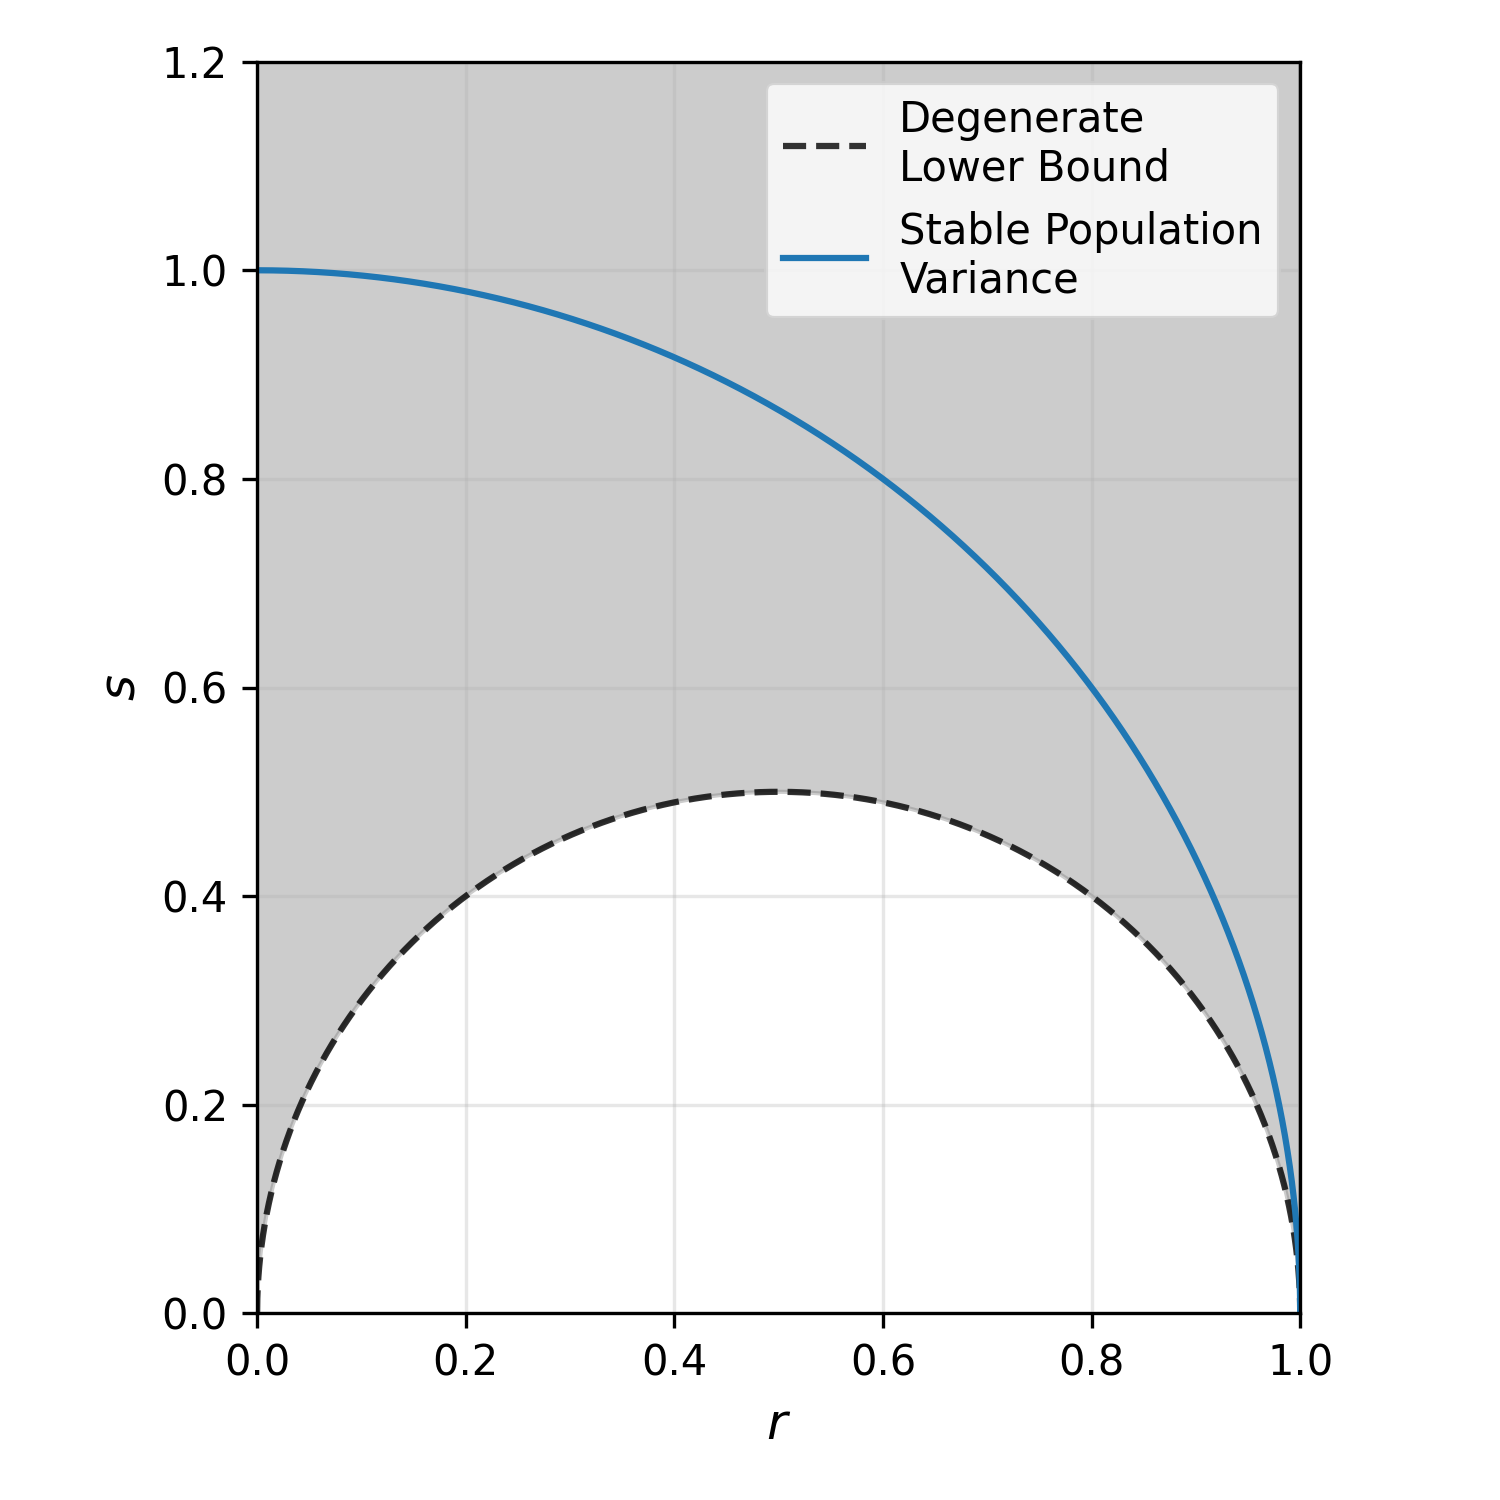
\includegraphics[width=2.8in]{figures/possible_r_rs.png}
\centering
\caption{Possible values for the regression and residual coefficients are given by the shaded area, which extends upwards for $s \rightarrow \infty$. The degenerate lower bound has $s > \sqrt{r(1-r)}$ and stable population variance has $s = \sqrt{1-r^2}$.}
\label{fig:possible_r_rs}
\end{figure}



\begin{enumerate}
\item In the first case: $r = r^2 + s^2$, there is no regression towards the mean relative to the population, i.e., a descendant has the same expected z-score as its ancestor:
\begin{equation}
\frac{\tilde{\mu}_{i+n}}{\sigma_{i+n}^2} = \frac{X_i}{\sigma_i^2} \ .
\label{eq:first_case}
\end{equation}
No regression towards the mean in the z-scores can be considered degenerate.
\item In the second case: $r > r^2 + s^2$, we have $r^2 + s^2 < 1$ by Eq. \ref{eq:r_require} and $\sigma_{i+n}^2 \rightarrow 0$ for large $n$, as is shown in section \ref{pvd}. Here, the marginal variance converges to zero faster than the conditional expectation does, causing the expected z-score to diverge:
\begin{equation}
\frac{\tilde{\mu}_{i+n}}{\sigma_{i+n}^2} = (\frac{r}{r^2+s^2})^n \frac{X_i}{\sigma_i^2} \rightarrow \infty \ .
\label{eq:second_case}
\end{equation}
As $X_i$ was arbitrary, all descendants' expected z-scores would diverge regardless of their ancestors' scores, which can be considered degenerate.
\end{enumerate}
Equations (\ref{eq:first_case} and \ref{eq:second_case}) are obtained by taking the ratio of Eqs. \ref{eq:d_mean} and \ref{eq:pop_var}.


%% CAD %%
\subsection{Conditional Ancestor Distribution} \label{cad}

A general expression can be obtained for the conditional distribution of an ancestor's score given its descendant's score, given by
\begin{equation}
X_{i-n}|X_i \sim \mathcal{N}( \tilde{\mu}_{i-n}, \tilde{\sigma}_{i-n}^2) \ ,
\label{eq:a_dist}
\end{equation}
with
\begin{equation}
\tilde{\mu}_{i-n} = (\frac{r}{r^2+s^2})^n X_i
\label{eq:a_mean}
\end{equation}
and
\begin{equation}
\tilde{\sigma}_{i-n}^2 = [1 - (\frac{r^2}{r^2+s^2})^n] \sigma_{i-n}^2 \ .
\label{eq:a_var}
\end{equation}

In order to remain consistent with our earlier notation, it will be easiest to think of the generation number of the ancestor as also $b = i - n$. That is, the ancestor existed at time $b$, which is $n$ generations \emph{before} the current time $i$. One way to obtain the distribution of $X_{i-n}|X_i$ is with Bayes' rule: $f(x_{i-n}|x_i) \propto f(x_{b+n}|x_b) f(x_b)$.
This is similar, though not identical, to finding the posterior distribution for $\mu$ of a normal distribution when the prior distribution for $\mu$ is normal. Then, a normal prior times the normal likelihood gives a normal posterior. However, because $X_{b+n}|X_b \sim \mathcal{N}(r^n X_b, \tilde{\sigma}_{b+n}^2)$, the $r^n$ term obfuscates the conjugate prior.

An alternative approach is to recognize that $X_{i-n}$ and $X_i$ form a bivariate normal distribution. Then, conditioning on $X_i$, we can use the following standard results for bivariate normals:
\begin{equation}
\mathrm{E}(X_{i-n}|X_i) = \mathrm{E}(X_{i-n}) + \frac{\mathrm{Cov}(X_{i-n}, X_i)}{\mathrm{Var}(X_i)}[X_i - \mathrm{E}(X_i)]
\end{equation}
and
\begin{equation}
\mathrm{Var}(X_{i-n}|X_i) = \mathrm{Var}(X_{i-n}) - \frac{[\mathrm{Cov}(X_{i-n}, X_i)]^2}{\mathrm{Var}(X_i)} \ .
\end{equation}
Plugging in Eqs. \ref{eq:pop_dist} - \ref{eq:pop_var} and Eq. \ref{eq:covariance}, we obtain the conditional ancestor distribution (CAD). This approach can also be used to confirm Eq. \ref{eq:d_dist}.

\subsection{One-step Upward Transition}
We can use Eqs. \ref{eq:a_dist} - \ref{eq:a_var} to obtain the one-step upward transition, i.e., the conditional distribution of a parent score given the child score:
\begin{equation}
X_{i-1}|X_i \sim \mathcal{N}( \tilde{\mu}_{i-1}, \tilde{\sigma}_{i-1}^2)
\label{eq:up_dist}
\end{equation}
with
\begin{equation}
\tilde{\mu}_{i-1} = \frac{r}{r^2+s^2} X_i
\label{eq:up_mean}
\end{equation}
and
\begin{equation}
\tilde{\sigma}_{i-1}^2 = \frac{s^2}{r^2+s^2} \sigma_i^2 \ .
\label{eq:up_var}
\end{equation}
This has a very similar form to the one-step downward transition (Eqs. \ref{eq:one_step} - \ref{eq:sigma_tilde}), only the coefficients have changed such that $r^2 + s^2$ is in the denominator.


% UPWARD CONVERGENCE
\subsection{Upward Convergence}

The CAD converges to the population distribution of $X_{i-n}$ for large $n$. This can be shown by first considering that $r < r^2 + s^2$ by the lower bound (Eq. \ref{eq:lower_bound}). Therefore, as $n \rightarrow \infty$,
\begin{equation}
(\frac{r}{r^2+s^2})^n \rightarrow 0 \ ,
\label{eq:conv_up_one}
\end{equation}
and by Eq. \ref{eq:a_mean},
\begin{equation}
\tilde{\mu}_{i-n} \rightarrow 0 \ .
\label{eq:conv_a_mean}
\end{equation}
%
Furthermore, $r^2 < r^2 + s^2$ as $r^2 < r$ by Eq. \ref{eq:r_require}. Therefore, as $n \rightarrow \infty$,
\begin{equation}
(\frac{r^2}{r^2+s^2})^n \rightarrow 0 \ ,
\label{eq:conv_up_two}
\end{equation}
and by Eq. \ref{eq:a_var},
\begin{equation}
\tilde{\sigma}_{i-n}^2 \rightarrow \sigma_{i-n}^2 \ .
\label{eq:conv_a_var}
\end{equation}
%
In summary, as $n \rightarrow \infty$:
\begin{equation}
X_{i-n}|X_i \sim X_{i-n} \ .
\label{eq:conv_a}
\end{equation}

This is another way of confirming the lower bound on $s$ (Eq. \ref{eq:lower_bound}), as the upward conditional expectation would not converge---as expected---under the degenerate condition.


\subsection{Role of the Coefficients in Upward Convergence} \label{role_up}
As with downward convergence, the rate at which the CAD converges to the population distribution is determined by the regression and residual coefficients in the same general ways. From Eqs. \ref{eq:a_mean} and \ref{eq:a_var}, it is clear that smaller $r$ means faster convergence, and vice versa; and that smaller $s$ means slower convergence, and vice versa. The ratio given by Eq. \ref{eq:conv_d_var_ratio} holds for the CAD (only with $i-n$ rather than $i+n$), which is clear from Eq. \ref{eq:a_var}.


% POPULATION VARIANCE DYNAMICS
\subsection{Stable and Unstable Population Variance} \label{pvd}

From Eq. \ref{eq:pop_var}, it is clear that if $r^2+s^2 < 1$ then $\sigma_{i+n}^2 \rightarrow 0$; whereas if $r^2+s^2 > 1$, then $\sigma_{i+n}^2 \rightarrow \infty$. These cases are called \emph{unstable population variance}. Such degenerate limits may be prevented if there were some negative feedback between $r$ or $s$ and $\sigma_i^2$. However, the resolution in this model is that $r^2+s^2 = 1$. Then, every generation has the same population variance, called \emph{stable population variance} (SPV). Formally, $\sigma_i^2 = 1 \ , \,\, \forall i \in \mathbb{N}$.

By the polygenic application, for the child generation to have the same population variance as the parent generation (see Eq. \ref{eq:one_step}), indeed for all generations to have the same population variance, it must be the case that  $r^2+s^2 = 1$.


% STATIONARY DISTRIBUTION
\subsection{Stationary Distribution}

The stationary distribution of the Markov model can be shown to have a couple of key properties.

\begin{enumerate}
%
\item \emph{SPV is a necessary and sufficient condition for the stationary distribution.} It is clear from section \ref{pvd} and Eq. \ref{eq:pop_var} that only under SPV, is $X_i \sim X_{i+n} \sim \mathcal{N}(0, 1) \ , \,\, \forall \, i, n \in \mathbb{N}$.

\item \emph{The stationary distribution is reversible.} It is clear comparing Eqs. \ref{eq:d_mean} and \ref{eq:d_var} to Eqs. \ref{eq:a_mean} and \ref{eq:a_var} that the model behaves identically going forwards and backward in time when there is SPV. That is, the CDD and CAD (Eqs. \ref{eq:d_dist} and \ref{eq:a_dist}) are identical under SPV:
\begin{equation}
\tilde{\mu}_{i-n} = \tilde{\mu}_{i+n} = r^nX_i
\label{eq:stable_mean}
%
\end{equation}
\begin{equation}
\tilde{\sigma}_{i-n}^2 = \tilde{\sigma}_{i+n}^2 = 1-r^{2n}
\label{eq:stable_var}
\end{equation}
%
\end{enumerate}



\subsection{Exponential Functions for Downward Convergence}

The role of the coefficients can also be seen in the equations for the rate of change over generations in the parameters of the CDD.

The rate of change in the conditional expectation is negative and increasing with $n$ (positive second partial derivative). That is, the conditional expectation asymptotically approaches zero by
\begin{equation}
\frac{\partial }{\partial n}[\tilde{\mu}_{i+n}] = -\log(\frac{1}{r}) \, \tilde{\mu}_{i+n}
\label{eq:partial_d_mean}
\end{equation}
where '$\log$' is the natural logarithm. Likewise, the rate of change in the ratio of the conditional variance to the marginal variance is positive and decreasing with $n$ (negative second partial derivative). The ratio asymptotically approaches one by
\begin{equation}
\frac{\partial }{\partial n}[\frac{\tilde{\sigma}_{i+n}^2}{\sigma_{i+n}^2}] = \log(1+\frac{s^2}{r^2}) \, [1 - \frac{\tilde{\sigma}_{i+n}^2}{\sigma_{i+n}^2}] \ .
\label{eq:partial_d_var}
\end{equation}
Equations (\ref{eq:partial_d_mean} and \ref{eq:partial_d_var}) confirm the remarks on $r$ and $s$ made in section \ref{role_down}. They also make it clear that we can rewrite Eqs. \ref{eq:d_mean} and \ref{eq:d_var} as the following exponential functions:
\begin{equation}
\tilde{\mu}_{i+n} = X_i \, \exp[-\log(\frac{1}{r}) \, n]
\label{eq:expo_d_mean}
\end{equation}
and
\begin{equation}
\tilde{\sigma}_{i+n}^2 = \sigma_{i+n}^2 \, (1 - \exp[-\log(1+\frac{s^2}{r^2}) \, n]) \ .
\label{eq:expo_d_var}
\end{equation}
These show that the parameters of the CDD exponentially converge on the parameters of the population distributions as the generation gap $n$ widens.


\subsection{Exponential Functions for Upward Convergence}

As with downward convergence, upward convergence has analogous equations, which similarly confirm the remarks on $r$ and $s$ made in section \ref{role_up}:
\begin{equation}
\frac{\partial}{\partial n}[\tilde{\mu}_{i-n}] = -\log(\frac{r^2 + s^2}{r}) \, \tilde{\mu}_{i-n}
\label{eq:partial_a_mean}
\end{equation}
%
\begin{equation}
\frac{\partial }{\partial n}[\frac{\tilde{\sigma}_{i-n}^2}{\sigma_{i-n}^2}] = \log(1+\frac{s^2}{r^2}) \, [1 - \frac{\tilde{\sigma}_{i-n}^2}{\sigma_{i-n}^2}]
\label{eq:partial_a_var}
\end{equation}
%
\begin{equation}
\tilde{\mu}_{i-n} = X_i \, \exp[-\log(\frac{r^2 + s^2}{r}) \, n]
\label{eq:expo_a_mean}
\end{equation}
%
\begin{equation}
\tilde{\sigma}_{i-n}^2 = \sigma_{i-n}^2 \, (1 - \exp[-\log(1+\frac{s^2}{r^2}) \, n]) \ .
\label{eq:expo_a_var}
\end{equation}
Therefore, there is also exponential convergence of the CAD as the generation gap $n$ widens.



% MOBILITY AND INFORMATION-LOSS
\section{Proposed Mobility Measure}

We would like to find some way to quantify the degree of \emph{intergenerational mobility} in the score of a descendant, given the score of its ancestor. This would also correspond to the \emph{loss of information} for predicting a descendant's score from its ancestor's score, or vice versa.

It may be noted that for the CDD, faster convergence means that it quickly becomes indistinguishable from the population distribution of its generation. The information provided by an ancestor's score that might predict its descendant's score is quickly \emph{lost} over the intervening generation(s). Faster convergence means greater mobility, in that within a small number of generations the CDD moves \emph{towards} the population distribution (both in expectation and variance). Likewise, for the CAD, faster convergence means that a descendant's score provides less information about its ancestor's score.

We have previously shown that convergence of the conditional distribution to the marginal distribution (both upward and downward) occurs faster with smaller $r$ and larger $s$, and vice versa. Accordingly, a simple measure of mobility and information-loss would be proportional to $s$ and inversely proportional to $r$.

\begin{definition}
Let $m$ be the measure of mobility, or equivalently of information-loss, for the Markov model with parameters $r$ and $s$, given by
\begin{equation}
m := \frac{s}{r} \ .
\end{equation}
\label{def:m}
\end{definition}

In general, a value of $m$ is not unique to a given formulation of the Markov model, because infinitely many values for $r$ and $s$ can have the same ratio. Although it is not investigated here, different Markov models with the same $m$ may have varied rates of convergence upwards or downwards in expectation or variance. However, \emph{under SPV, $m$ fully parametrizes the Markov model} (by uniquely determining $r$ and $s$).

It is straightforward to show that under the various limits of $r$ and $s$, the desired effects in mobility and information-loss occur, consistent with the proposed measure of mobility. If $r \rightarrow 0$ or $s \rightarrow \infty$ then rapid convergence both upward and downward occur, consistent with the proposed $m \rightarrow \infty$. Interestingly, in the case where $s \rightarrow 0$, then either $r \rightarrow 0$ or $r \rightarrow 1$ by Eq. \ref{eq:lower_bound} (see Fig. \ref{fig:possible_r_rs}). In the former, $r$ shrinks faster than $s$ does, causing $m \rightarrow \infty$, and the CDD and CAD rapidly converge. In the latter combination of $r$ and $s$, $m \rightarrow 0$, and no convergence occurs in the CDD and CAD.

%\newpage

% ASSUMPTIONS AND LIMITATIONS
\section{Application for Modeling a Polygenic Trait}

The Markov model proposed in this paper has features that should be noted for its application to model a polygenic trait, such as height.

\subsection{Assumptions and Limitations} \label{al}

Assumptions of the model:
\begin{enumerate}
\item Normal distribution of the polygenic trait in the population, verified for human height \cite{preece}.
\item Normal linear relationship between parent and child scores, verified for human height \cite{luo}.
\item The probability of successful reproduction for all members of the population is the same for all scores, i.e., no natural selection takes place.
\item The SD of the conditional child distribution is proportional to the marginal SD of the parent generation (Eq. \ref{eq:sigma_tilde}), though this assumption vanishes under SPV and $s$ merely becomes the ratio of the conditional child distribution to the population distribution.
\end{enumerate}
Limitations of the model:
\begin{enumerate}
\item Generations of the population exist in discrete time and are non-overlapping.
\item Changes in population size are not described.
\item Only the relationship between a single ancestor-descendant pair is modeled, such as mother and daughter or grandfather and granddaughter. Mating partners and other ancestors are unaccounted for.
\end{enumerate}

\subsection{Adjustment for Uniform Environmental Effects} \label{adjustment}

The model described thus far does not describe the average movement of the population mean between generations as a result of external effects that would uniformly shift the conditional mean of each child. This has occurred in human height, which increased between generations in developed countries during the 19th and 20th centuries, an observation that has been attributed to population-wide improvements in the environment for growth, relating to nutrition and health \cite{bogin, perkins}.

Such effects can easily be included in the model. Denoting the uniform increase in height between generations by $c$, we have
\begin{equation}
X_1|X_0 \sim \mathcal{N}(\mu_i + c + r \, (X_i - \mu_i), \, s^2 \sigma_i^2) \ ,
\label{eq:unif_env}
\end{equation}
Then, the only change to the model is in the population mean, which is given by $\mu_{i \pm n} = \mu_i \pm n c$, if $c$ is constant between generations. Alternatively $c$ could vary between generations as a function of time, which is also easy to parametrize.


\subsection{Estimation of Parameters} \label{estimation}

The regression and residual parameters can be estimated with a normal linear model from one-step transition data, which consists of the paired heights of parents and children. When handling this data, the parent and child scores are standardized to the sample mean and SD of the measured parent scores, to match the form of the model. Then, the vector of coefficients $\beta = (c, r)$ is given by Eq. \ref{eq:unif_env} and is estimated through ordinary least squares. That is, in a plot of parent versus child scores, the estimate for $c$ is the intercept and the estimate for $r$ is the slope of the regression line. Additionally, the unbiased estimate of $s$ is obtained from $\sqrt{RSS / (n-p)} \,$, where $p = 2$ and RSS is the residual sum of squares.


The regression and residual coefficients provide the SD ratio of the child-generation population to the parent-generation population through the following relation: $\mathrm{SD}\,\, \mathrm{ratio} =  \sqrt{r^2+s^2}$ (see Eq. \ref{eq:pop_var}). Therefore, having estimates of any two of the three terms immediately provides an estimate of the third. Furthermore, if SPV can be assumed, then estimating either $r$ or $s$ immediately yields an estimate of the other. It is worth noting that under SPV, $r$ is also the correlation coefficient between parent and child scores (see Eq. \ref{eq:covariance}). Estimates of $r$ and $s$ are important because they parametrize the entire model.



%% MODEL VERIFICATION FOR HUMAN HEIGHT %%
\section{Model Verification for Human Height}

From two large datasets on the heights of parents and their children, the proposed model is verified through statistical tests for the one-step transition, and the regression and residual coefficients are estimated.

\subsection{Requirements for Model Verification} \label{verify}

All of the properties of the Markov model follow from the initial condition and the one-step downward transition, thus confirming their accuracy confirms the model properties. Model verification then consists of two parts:
\begin{enumerate}
\item The parental heights are modeled by the initial condition.
\item The conditional distribution of the adult child heights is modeled by the one-step downward transition.
\end{enumerate}



\subsection{Swedish Dataset}

The study \emph{Target Height as Predicted by Parental Heights in a Population-Based Study}, published in \emph{Nature---Pediatric Research} \cite{luo}, used a normal linear model to predict the heights of adult children from the heights of their parents from a large sample ($n = 2402$) of normal Swedish children born in the 1970s.

The authors did not report on the normality of the parental heights in the dataset but cited a paper that claims height is normally distributed in a population \cite{preece}. A uniform increase in height between generations was observed between the parent and child generations, amounting to 0.7 cm for male and 1.0 cm for female subjects.

The authors confirmed the validity of a normal linear model for the one-step transition of parent to child heights through the following tests:
\begin{enumerate}
\item The residuals were normally distributed (tested by skewness and kurtosis).
\item The mean residual values were fairly constant over the range of midparental heights, fluctuating around zero, and were only statistically significantly above zero ($p < 0.05$) for very short midparental heights (below -2 SDs).
\item The mean residual values were constant over the range of difference in parental heights.
\item The residual SDs were constant over the range of midparental heights.
\item The residual SDs were constant over the range of difference in parental heights.
\end{enumerate}

Varied values of $r$ and $s$ were estimated by least squares for using mothers' heights to predict sons' heights, fathers' heights to predict sons' heights, mothers' heights to predict daughters' heights, etc. These four possibilities averaged $r = 0.49$ and $s = 0.88$, which essentially produces SPV, producing by Eq. \ref{eq:pop_var} an SD ratio of 1.01. The observed SD ratio was 0.978 for fathers and sons, and 1.16 for mothers and daughters, somewhat consistent with SPV.


\subsection{English Dataset} \label{pearson}

Karl Pearson organized the collection of the heights of mothers, fathers and their adult children on over 1,100 families in England in the 1890s, with no more than two adult children per family \cite{pearson}. The model was verified (by section \ref{verify}) for the mother-daughter data ($n = 1375$) with statistical tests at the 5\% level (see section \ref{links}). The data was standardized as described in section \ref{estimation}. The mother's scores were normally distributed, passing the skewness, kurtosis, and D'Agostino's normality tests, and normality was also clear from a Q-Q plot. The normality of the residuals and of the daughter generation was confirmed by the same methods. As in the Swedish data, an increase in height (3.3 cm) between generations was observed, therefore the adjustment of section \ref{adjustment} was made. The residuals were uncorrelated with the parent scores, as shown in Fig. \ref{fig:pearson_residuals_by_score}. Therefore, the adjustment constant was valid as the 3.3 cm shift was uniform for all children.

\begin{figure}[h]
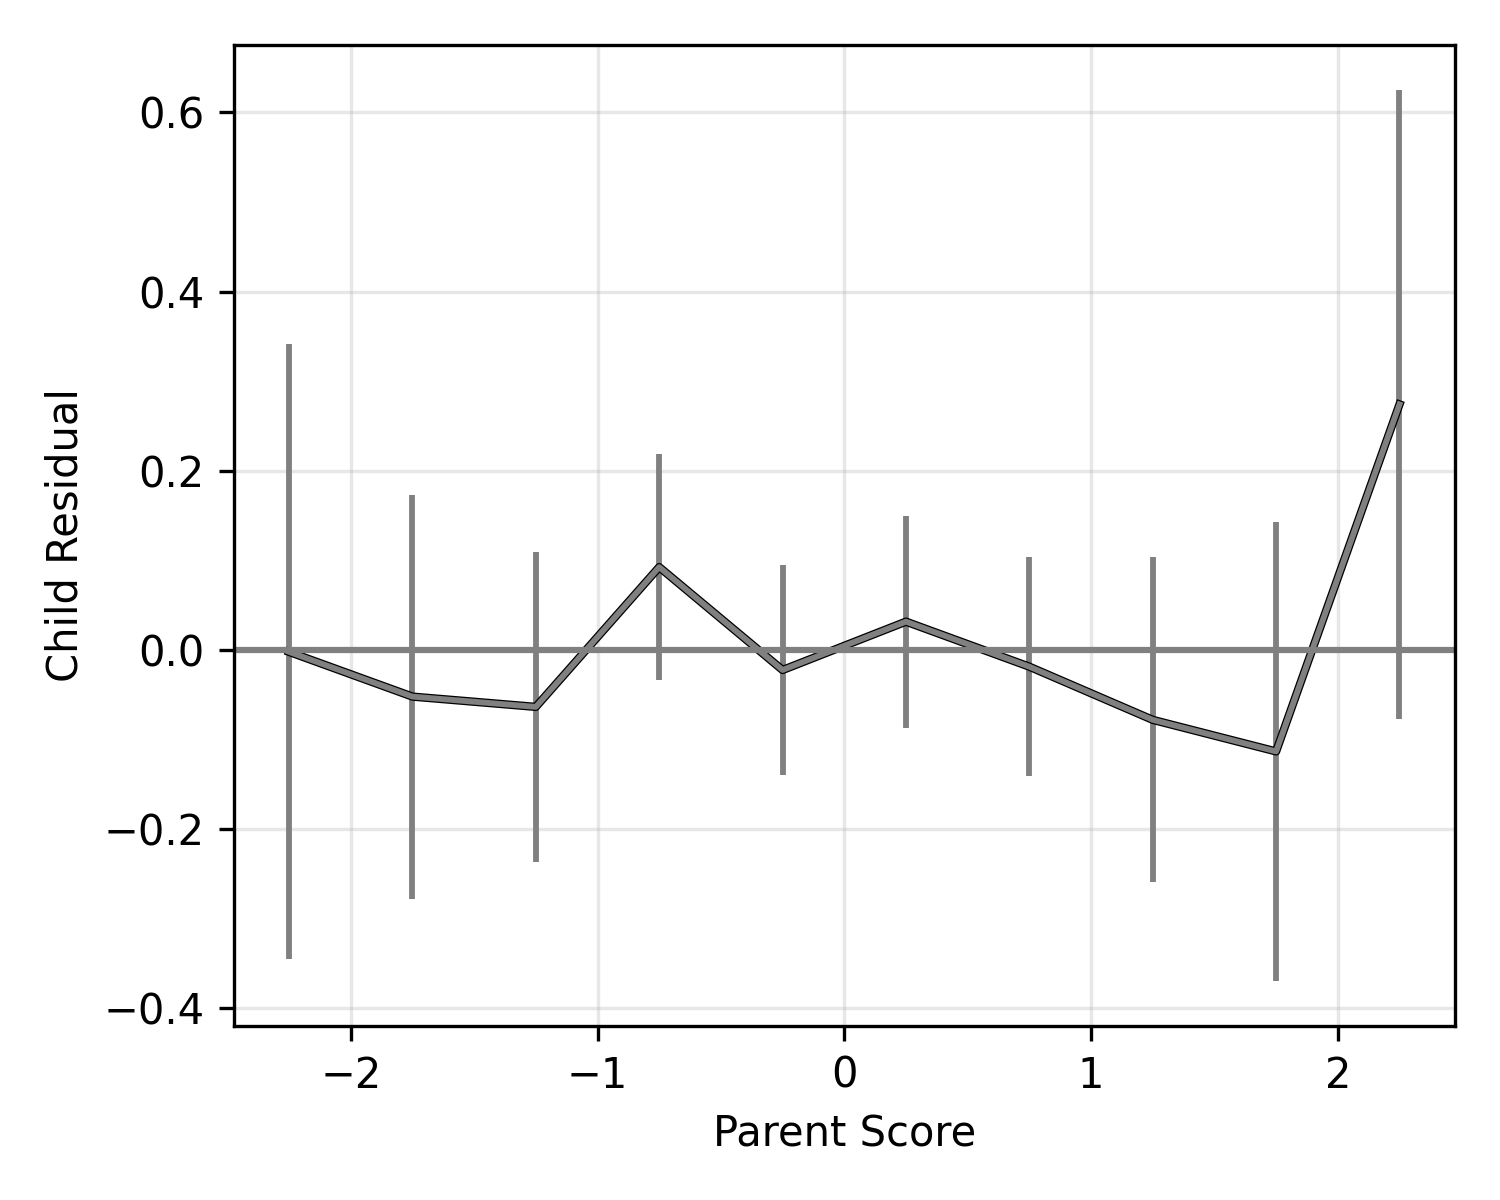
\includegraphics[width=2.8in]{figures/pearson-lee-mother-daughter-residuals_by_parent.png}
\centering
\caption{Mean values of the residuals by parent score, with normal 95\% confidence intervals for the Pearson mother-daughter data \cite{pearson}.}
\label{fig:pearson_residuals_by_score}
\end{figure}

Though not shown here, the same statistical tests were applied to the father-son data ($n$ = 1078). All tests passed except the kurtosis and D'Agostino's tests for normality of the residuals and of the son generation. The failures occurred because of deviations from normality in the edges of the residuals and of the son generation (more than two standard deviations from the mean) as apparent from their Q-Q plots.

The Pearson female data had the estimates $r = 0.54$ and $s = 0.96$ (by section \ref{estimation}), which nearly produce SPV (SD ratio of 1.10). The female data failed the F-test for equality of variances between the mother and daughter generation ($p < 0.001$). The Pearson male data had the estimates $r = 0.51$ and $s = 0.89$, which nearly produce SPV (SD ratio of 1.03). The male data passed the F-test for equality of variances between the father and son generation ($p = 0.20$).

\newpage

\subsection{Stable Population Variance for Height}

We have confirmed from the Pearson female data both the initial condition and the one-step downward transition, and thus the entire model---as long as there is SPV. This is because, under SPV, the assumption of proportionality between residual and population variance of the previous generation vanishes, as described in assumption 4 of section \ref{al}.

Overall, SPV seems \emph{a priori} to be a reasonable condition for human height (e.g. continually increasing variance over generations would eventually lead to absurdly large differences in height between the tallest and shortest members of the population). One possible explanation for why the SD ratios were sometimes larger than one is that the adult children tended to be younger than their parents. Therefore, the adult child heights may have continued to regress towards the mean after the studies. In the Swedish data, all of the adult children had their heights measured at around age eighteen \cite{karlberg}. Similarly, in the Pearson data, all of the adult children were at least age 18 years old, and all of the parents were at most 65 years old \cite{pearson}.

% PERCENTILE TRANSITION MATRICES
\section{Percentile Transition Matrices}

Percentile transition matrices make interpretable predictions over generations, enabling visualizations of multi-generational regression towards the mean and the effects of the mobility measure.

\subsection{Formulation} \label{formulation}

The calculations of attributable and destined probabilities can be defined by percentile sets. For example, in $P_{\delta , n}(Q_j | Q_k)$, the percentile set $Q_k$ would be converted to a real number set through the cdf $F_i^{-1}(Q_k)$, using the marginal variance $\sigma_i^2$. It should be noted that when attributable and destined probabilities are simulated this way, they are not affected by unstable population variance because using percentiles is a way of standardizing to different variances.

Percentile transition matrices result from equal-size, continuous percentile sets $Q_1$, $Q_2$, ..., $Q_m$. For example, for $m=5$, we have: $Q_1 = \left(0, 0.2\right]$, $Q_2 = \left(0.2, 0.4\right]$, ..., $Q_5 = \left(0.8, 1\right]$. As all percentile sets have the same size, e.g., $P_{\cdot}(Q_j) = P_{\cdot}(Q_k) = 0.2$, the calculations can be equivalently interpreted as attributable and destined probabilities. That is, we have
\begin{equation}
P_{\alpha , n}(Q_j | Q_k) = P_{\delta , n}(Q_j | Q_k) = P_{\cdot , n}(Q_j | Q_k)
\label{eq:ad_eq}
\end{equation}
$\forall j, k \in \{1, 2, \dots , m\}$.


\begin{definition}
Let a percentile transition matrix be given by
\begin{equation}
\mathcal{P}(i, n, m) :=
\begin{pmatrix}
P_{\cdot , n}(Q_m | Q_1) &  P_{\cdot , n}(Q_m | Q_2)  & \ldots & P_{\cdot , n}(Q_m | Q_m)\\
P_{\cdot , n}(Q_{m-1} | Q_1)  &  P_{\cdot , n}(Q_{m-1} | Q_2) & \ldots & P_{\cdot , n}(Q_{m-1} | Q_m)\\
\vdots & \vdots & \ddots & \vdots\\
P_{\cdot , n}(Q_1 | Q_1)  &   P_{\cdot , n}(Q_1 | Q_2)       &\ldots & P_{\cdot , n}(Q_1 | Q_m)
\end{pmatrix}
\label{eq:ptm}
\end{equation}
where $Q_1, Q_2, \dots , Q_m$ are continuous, equal-size percentile sets of size $1/m$, such that
\begin{equation}
P_u(Q_j) = \frac{1}{m}
\label{eq:size}
\end{equation}
$\forall j \in \{1, 2, \dots , m\}$ and $\forall u \in \{i, n\}$, where $P_u(Q_j)$ is the marginal probability of $X_u \in F_u^{-1}(Q_j)$.
\label{def:ptm}
\end{definition}


\subsection{Persymmetry} \label{persymmetry}

Percentile transition matrices are persymmetric, i.e., symmetric along the northeast to southwest diagonal. This results from Eq. \ref{eq:set_set_eq}, where if $Q_j$ and $Q_k$ have the same size, we get the persymmetry property
\begin{equation}
P_{ \cdot, n}(Q_j | Q_k) = P_{\cdot, n}(Q_k | Q_j) \ .
\label{eq:persymmetry}
\end{equation}
Persymmetry says, for example, that the probability relating a parent in the bottom quintile to a child in the second quintile is the same as that relating a parent in the second quintile to a child in the bottom quintile.


\subsection{Symmetry}

Percentile transition matrices are symmetric, i.e., symmetric along the northwest to southeast diagonal. This results from the fact that normal distributions are symmetric, which means that
\begin{equation}
f_d(-x_{i+n} | -x_i) f_m(-x_i) = f_d(x_{i+n} | x_i) f_m(x_i) \ .
\label{eq:normal_symmetry}
\end{equation}
It is also trivially true that
\begin{equation}
f_a(x_i | x_{i+n}) f_m(x_{i+n}) = f_d(x_{i+n} | x_i) f_m(x_i) = f(x_{i+n} , x_i)
\label{eq:trivial}
\end{equation}
where $f_a(x_{i+n}|x_i)$ is the conditional pdf of the CAD (Eq. \ref{eq:a_dist}).
Combining Eqs. \ref{eq:normal_symmetry} and \ref{eq:trivial}, we get
\begin{equation}
f_d(x_{i+n}|x_i)f_m(x_i) = f_a(-x_i|-x_{i+n})f_m(-x_{i+n}) \ ,
\end{equation}
which leads immediately by Eqs. \ref{eq:state_set} and \ref{eq:set_set} to the symmetry property
\begin{equation}
P_{ \cdot, n}(Q_j, Q_k) = P_{\cdot, n}(Q_{m-k+1}, Q_{m-j+1}) \ .
\label{eq:symmetry}
\end{equation}
Symmetry says, for example, that the probability relating parents in the bottom quintile to children in the fourth quintile is the same as that relating parents in the second quintile to children in the top quintile.

\subsection{Bisymmetry and Number of Unique Entries} \label{bisymmetry}

Percentile transition matrices are bisymmetric, i.e, symmetric along both diagonals, which we just showed. A result of bisymmetry is that the number of unique entries in a percentile transition matrix is $m + (m-2) + ... + 4 + 2$ for even $m$, and $m + (m-2) + ... + 3 + 1$ for odd $m$. This is clear by the following argument: filling in the entries by row, the number of entires in a row that have already been seen is twice the row index (starting at zero). Then, the first row has $m$ unique entries, the second row has $m-2$ unique entries, etc. By the arithmetic series, the number of unique entries is $m(m+2)/4$ for even $m$ and for $(m+1)^2/4$ for odd $m$.



\section{Visualizations of Percentile Transition Matrices} \label{visuals}

Percentile transition matrices were simulated from the model as well as estimated (through proportions) from observed data, enabling comparisons to the model. The matrices are visualized with the rows indicated by color, and the sizes proportional to the probabilities in Figs. \ref{fig:quintile_pearson} - \ref{fig:quintile_chetty}. The integral in Eq. \ref{eq:set_set} could not be solved analytically and was instead calculated numerically to very high fidelity (see section \ref{links}).

The simulated \emph{quintile}-transition matrices ($m = 5$) have 9 unique entries (see section \ref{bisymmetry}). One way to understand these figures is to consider an entry as a proportion of its column sum (probability destined) or row sum (probability attributable). Because of the symmetry property, the simulated matrices can equivalently be re-written with the x-axis as \emph{Descendant's Quintile}, and the y-axis as \emph{Cumulative Probability of Ancestor's Quintile}.


\subsection{Comparison to Pearson Data}

The observed percentile transition matrices of the Pearson mother-daughter and father-son data are shown along with a simulation from the estimated parameters in Fig. \ref{fig:quintile_pearson}. A reasonable similarity is observed between the simulated and observed matrices. It should be noted that there was a relatively small number of observations for each entry in the estimated matrices (minimum of 10, average of 49, and maximum of 149). This may explain some of the deviations between the male and female matrices, and potentially, the deviations from the simulated matrix.

The rightmost column in Fig. \ref{fig:quintile_pearson} shows that for height, a parent in the top quintile has about a 43\% chance of having a child also in (destined for) the top quintile, a 25\% chance of having a child in the fourth quintile, and so on. Equivalently, by Eq. \ref{eq:ad_eq}, these numbers can be interpreted as follows: about 43\% of the children in the top quintile are attributable to a parent also in the top quintile, about 25\% of the children in the fourth quintile are attributable to a parent in the top quintile, and so on.


\subsection{Multigenerational Regression Towards the Mean}

Between the Swedish and English datasets, the estimates for $r$ were about 0.5, with approximate SPV. Using $r = 0.5$ and SPV ($s \approx 0.866$), quintile transition matrices were simulated. These are shown in Fig. \ref{fig:quintile_stable} the regression towards the mean that takes place over multiple generations. The exponential downward convergence can be seen in the asymptotic approach of the probabilities towards uniform 20\%, with slowing rates of convergence as the generation-gap widens.


\subsection{Visualization of the Mobility Measure: The Case of US Family Income Mobility}

A quintile transition matrix relating the family incomes of 9,867,736 US children born between 1980-82 and their parents was simulated from income tax data by Chetty et al. and is reproduced in Fig. \ref{fig:quintile_chetty} \cite{chetty}. This transition matrix is crucially different than the other ones shown in this paper because it relates measures of the \emph{families} of children and their parents, rather than relating measures of an individual child to one of its parents (of the same sex). Nonetheless, reasons for similarity can be explained by the fact that the distribution of income can be approximated by a log-normal distribution \cite{battistin, neal}. Then, if the relation between the (log) income of parents and their children can be roughly approximated by a normal linear model, the Markov model described in this paper could reasonably be applied.

The effect of the mobility measure (Def. \ref{def:m}) is visualized in quintile transition matrices over varying $m$ in Fig. \ref{fig:quintile_mobility} under SPV, in which $m$ uniquely determines $r$ and $s$.

\begin{figure}[H]
\centering
%\advance\leftskip-0.4in
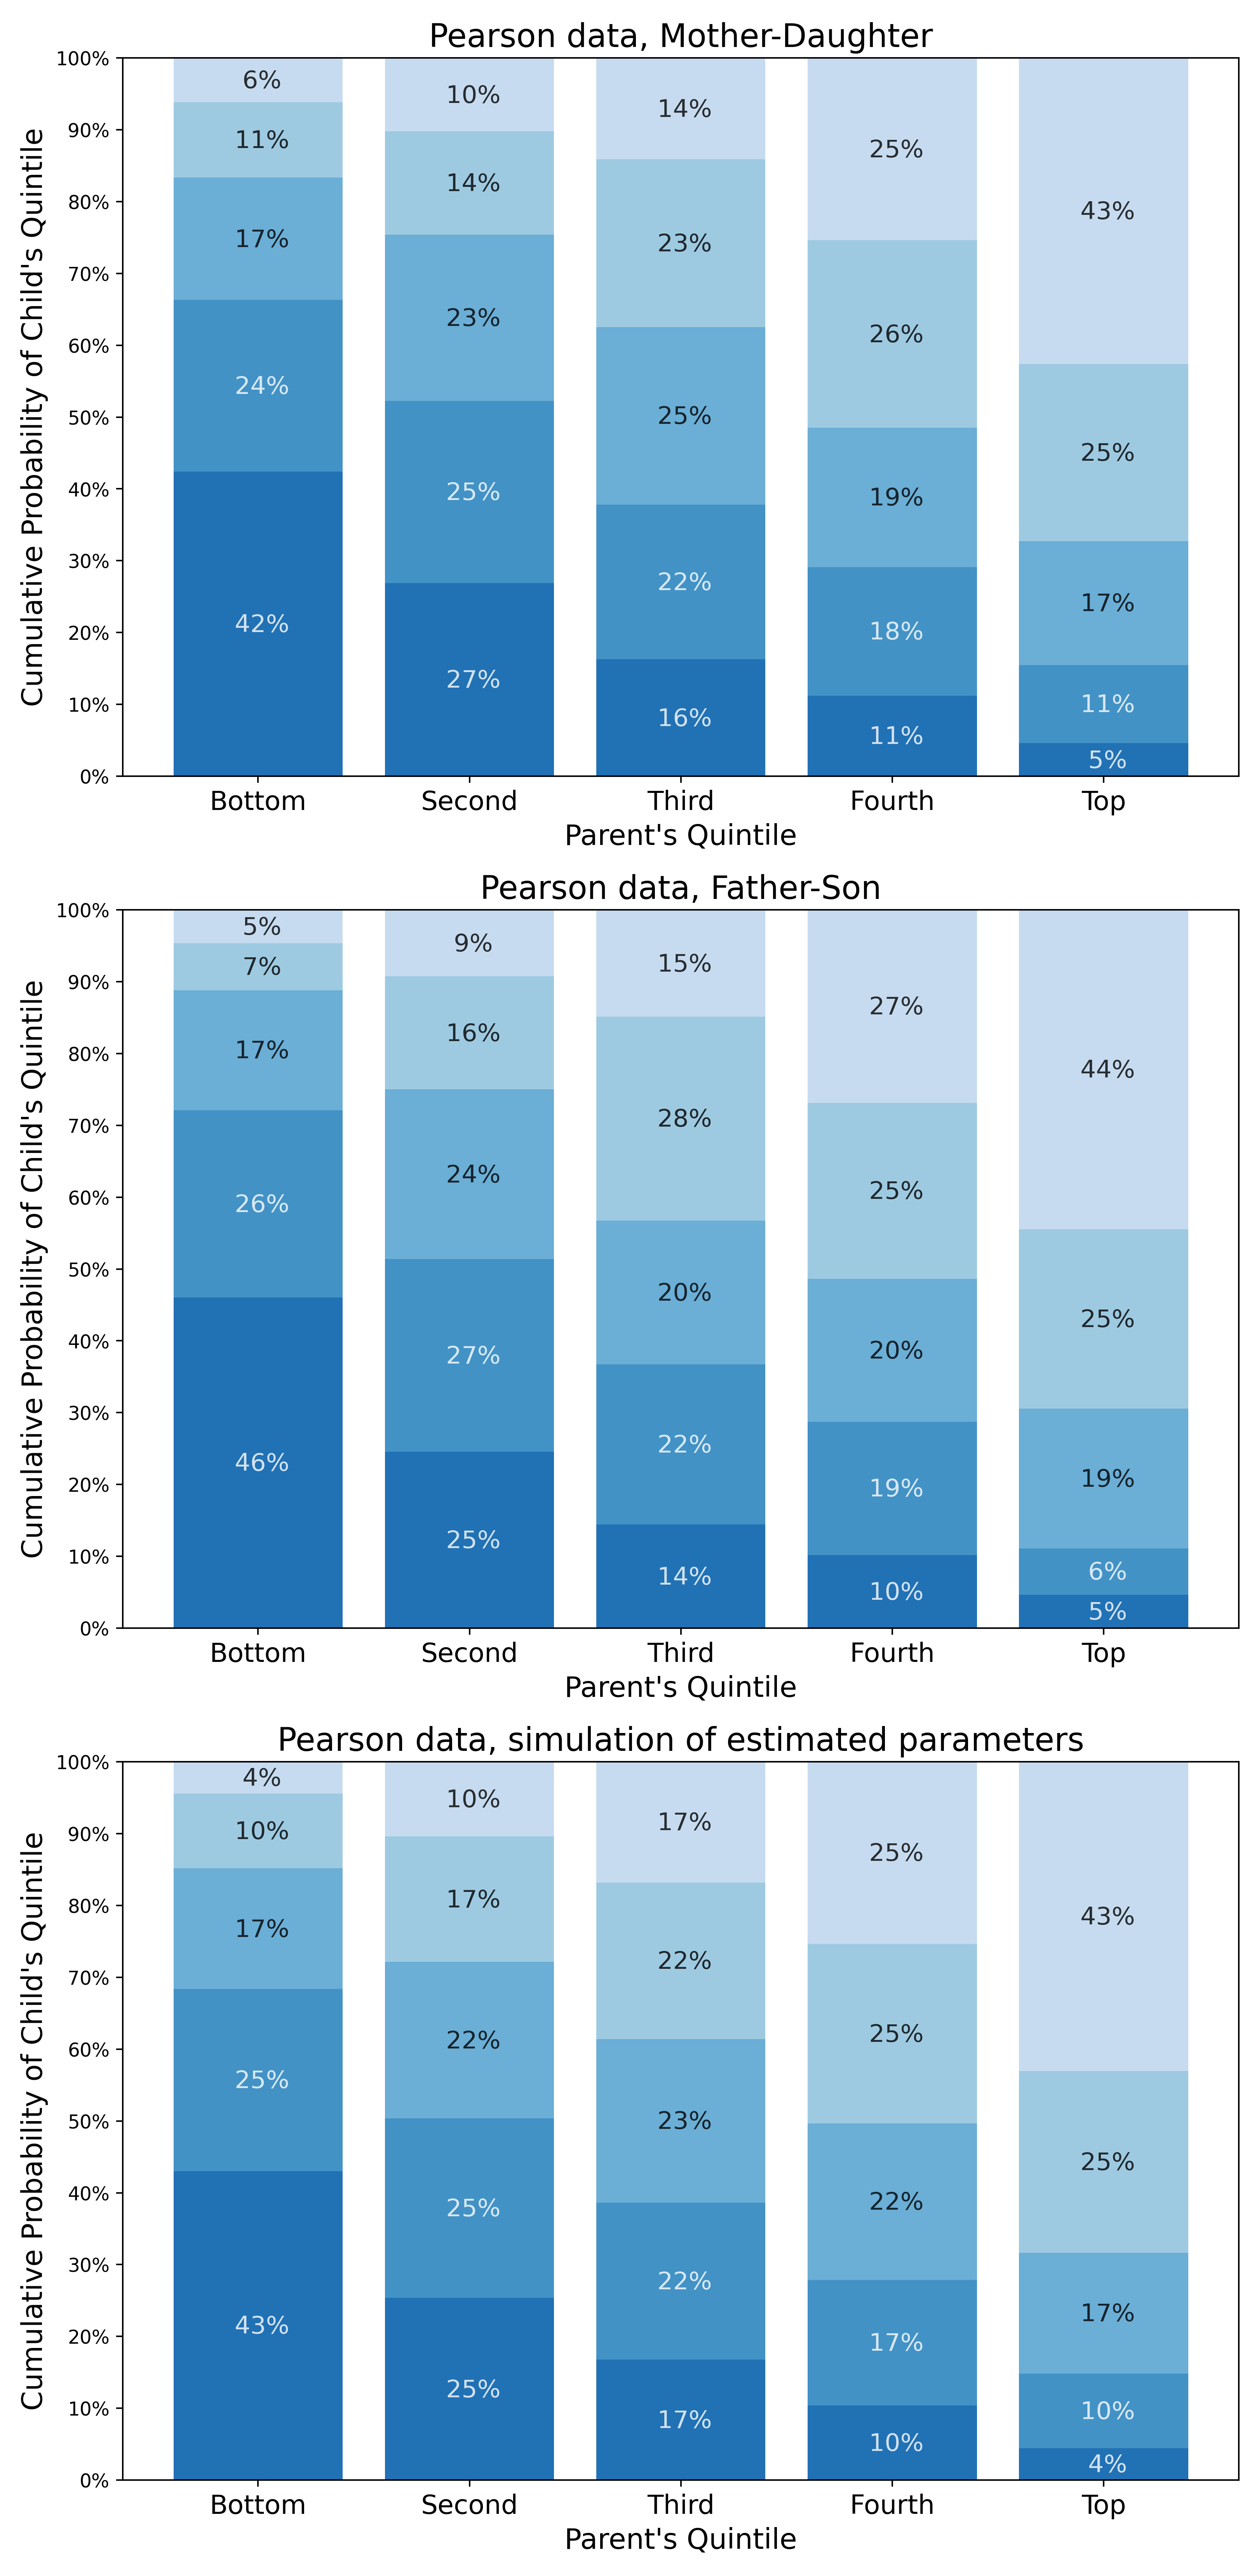
\includegraphics[width=2.8in]{figures/quintile-pearson.png}
\caption{Estimated and simulated quintile transition matrices from the Pearson data, with parameters $r = 0.54$, $s = 0.96$ for female and $r = 0.51$, $s = 0.89$ for male (see section \ref{pearson})  \cite{pearson}. These parameters result in identical simulated matrices (to the first decimal place), therefore only one is shown.}
\label{fig:quintile_pearson}
\end{figure}

Using the parent's family income to predict the child's income might be expected to increase the correspondence (and reduce mobility) due to the added predictive power of using both parent's incomes. On the other hand, predicting the child's family income might be expected to reduce the correspondence (and increase mobility), due to regression towards the mean. These effects are generally unknown, thus the caveat must be made that the transition matrix in Fig. \ref{fig:quintile_chetty} cannot be equivalently compared to the other transition matrices shown in this paper. Nonetheless, it can be generally remarked that there is a greater degree of observed mobility in family income (Fig. \ref{fig:quintile_chetty}) than in height (Fig. \ref{fig:quintile_pearson}). The mobility measure for income appears to be best approximated by $m \approx 3$ (see Fig. \ref{fig:quintile_mobility}). This can be compared with the mobility in height of about $m \approx$ 1.7-1.8, obtained from the estimates of the regression and residual coefficients.



\begin{figure}[H]
\centering
\advance\leftskip-0.16 in
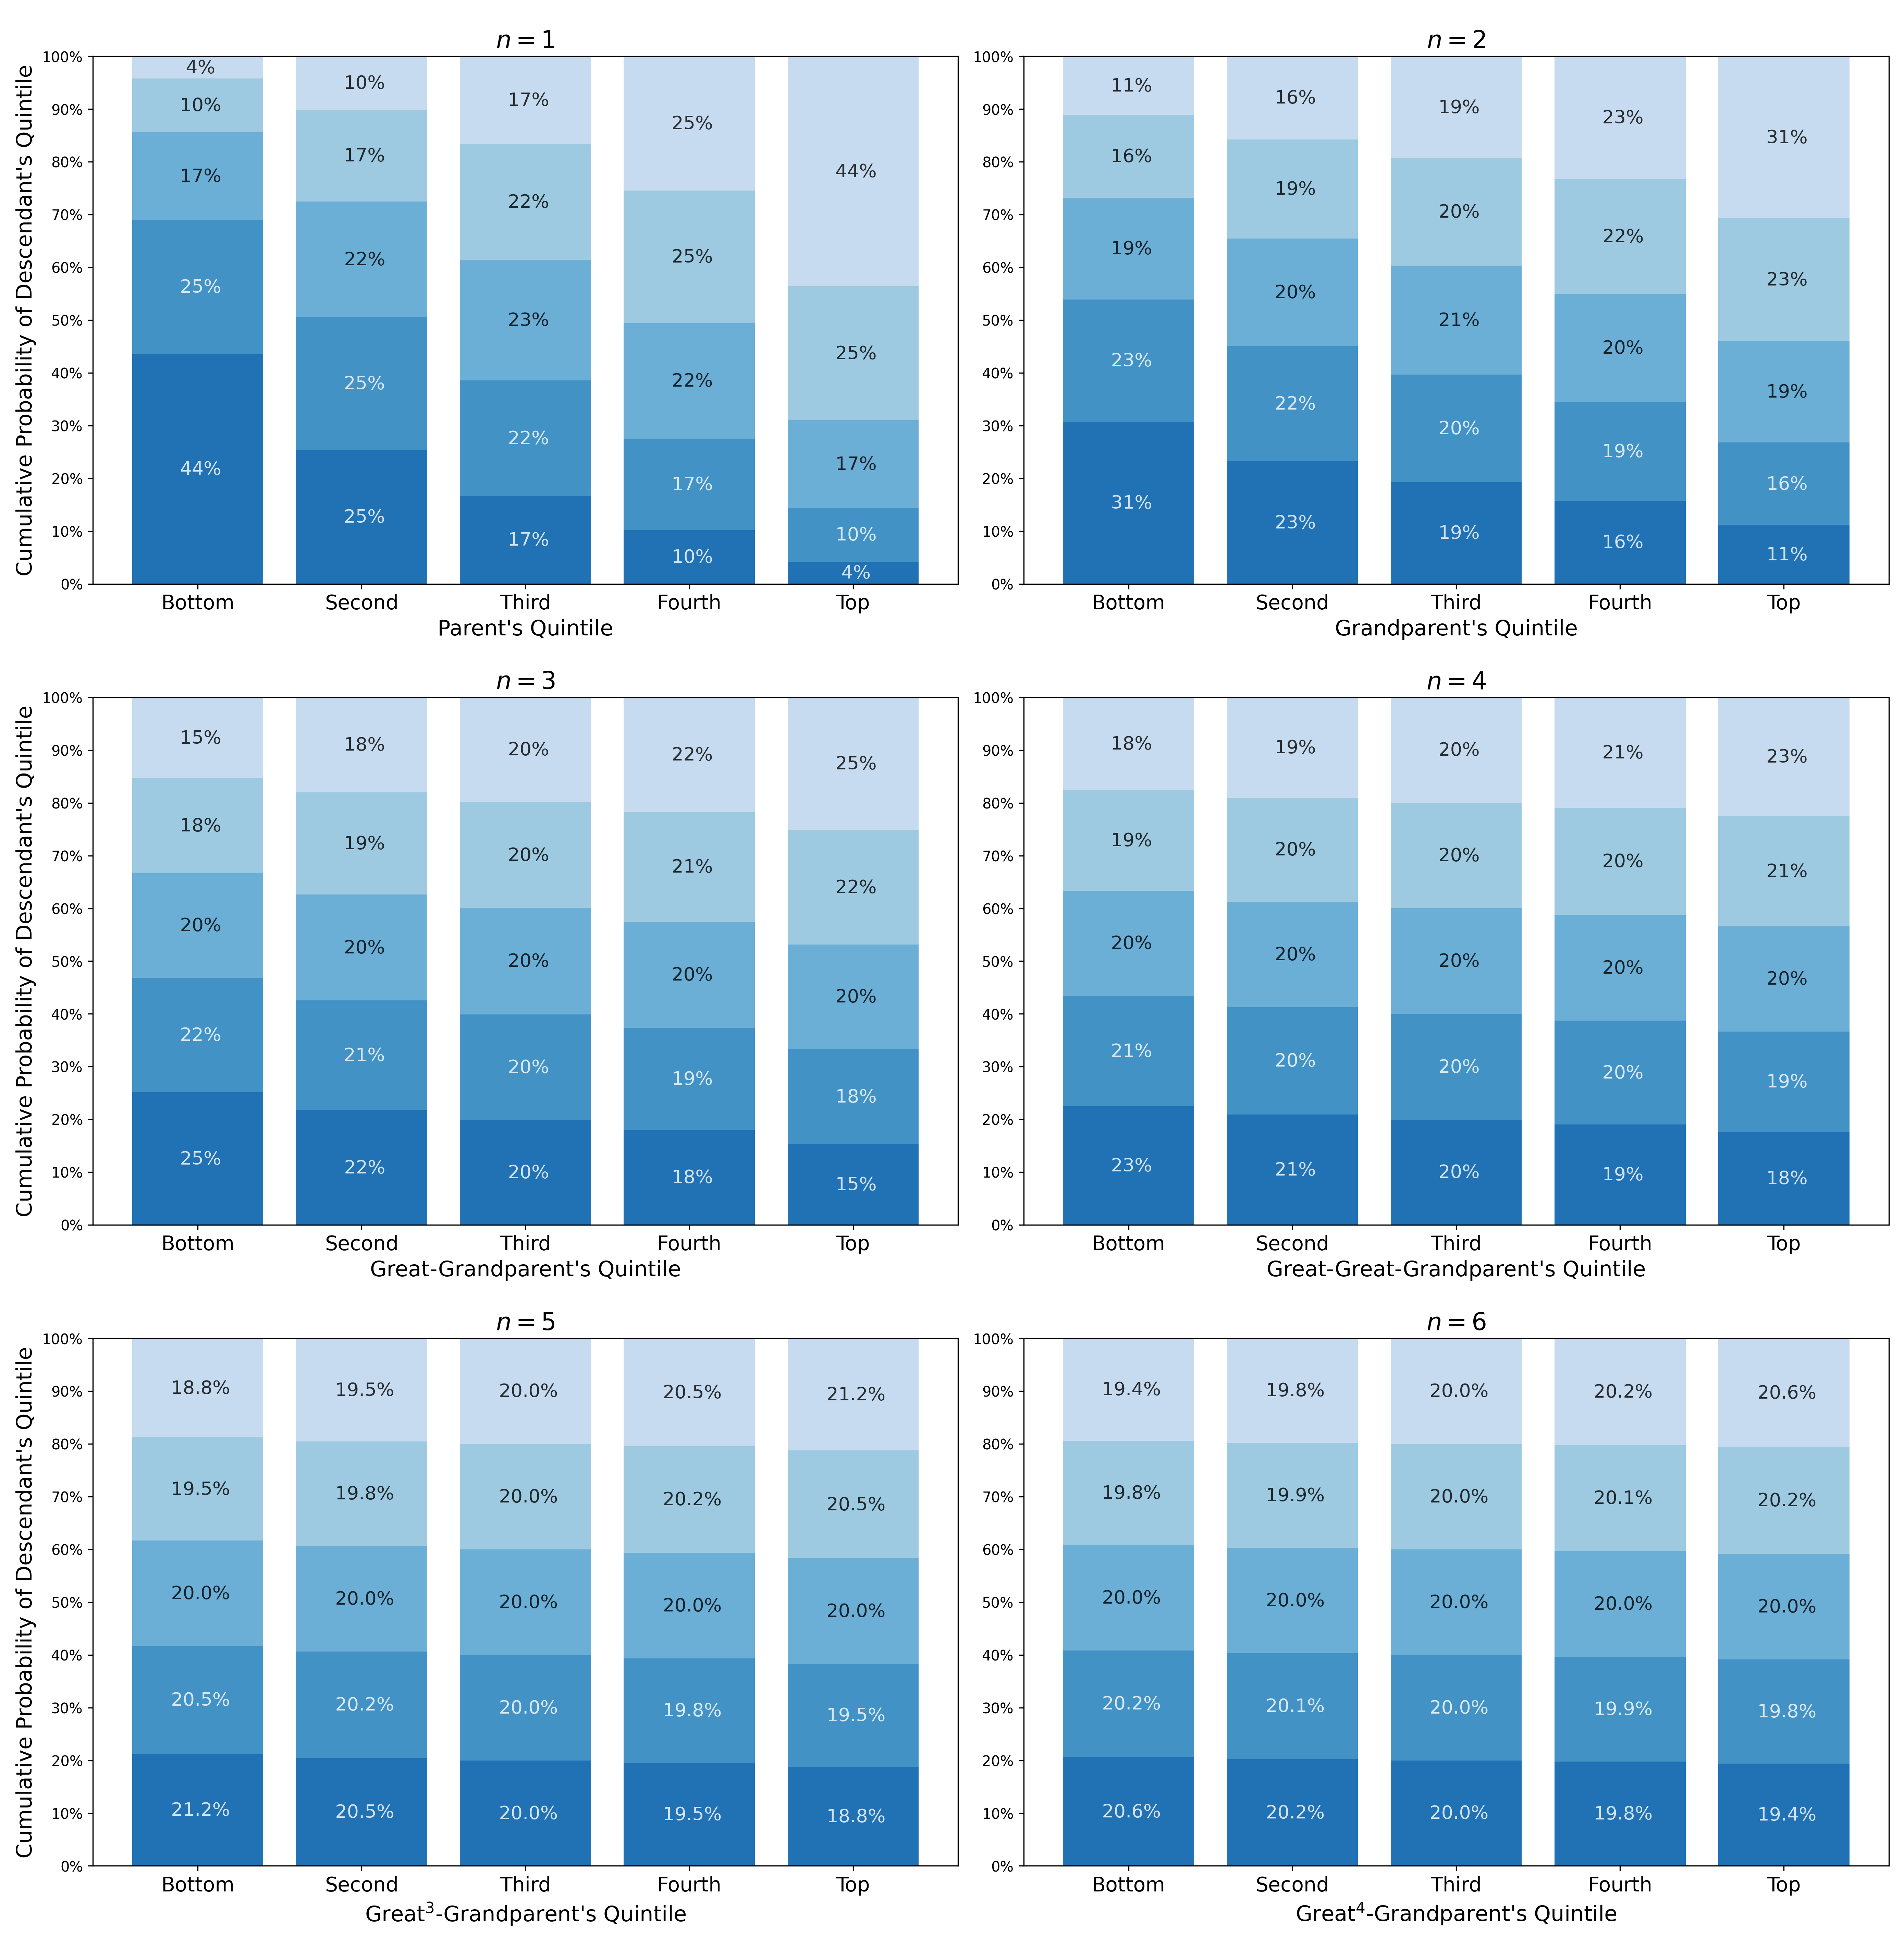
\includegraphics[width=5.2in]{figures/quintile-stable.png}
\caption{Quintile transition matrices over generation-gaps $n$ from 1 through 6, with SPV: $r = 0.5$ ($s \approx 0.866$).}
\label{fig:quintile_stable}
\end{figure}

The heritability of height has been well established \cite{luo, preece, wood}, though much of the correspondence between the incomes of parents and their children may be due to environmental factors. Nonetheless, studies of genome-wide SNPs have identified polygenic scores that account for a small amount ($\sim 2.5$\%) of the variance in family socioeconomic status (SES), including income \cite{trzaskowski, krapohl}. A normal linear model (and the corresponding Markov model introduced here) may be useful to describe both the genetic \emph{and} environmental factors that relate the incomes of parents and their children.



\begin{figure}[H]
\centering
\advance\leftskip-0.16 in
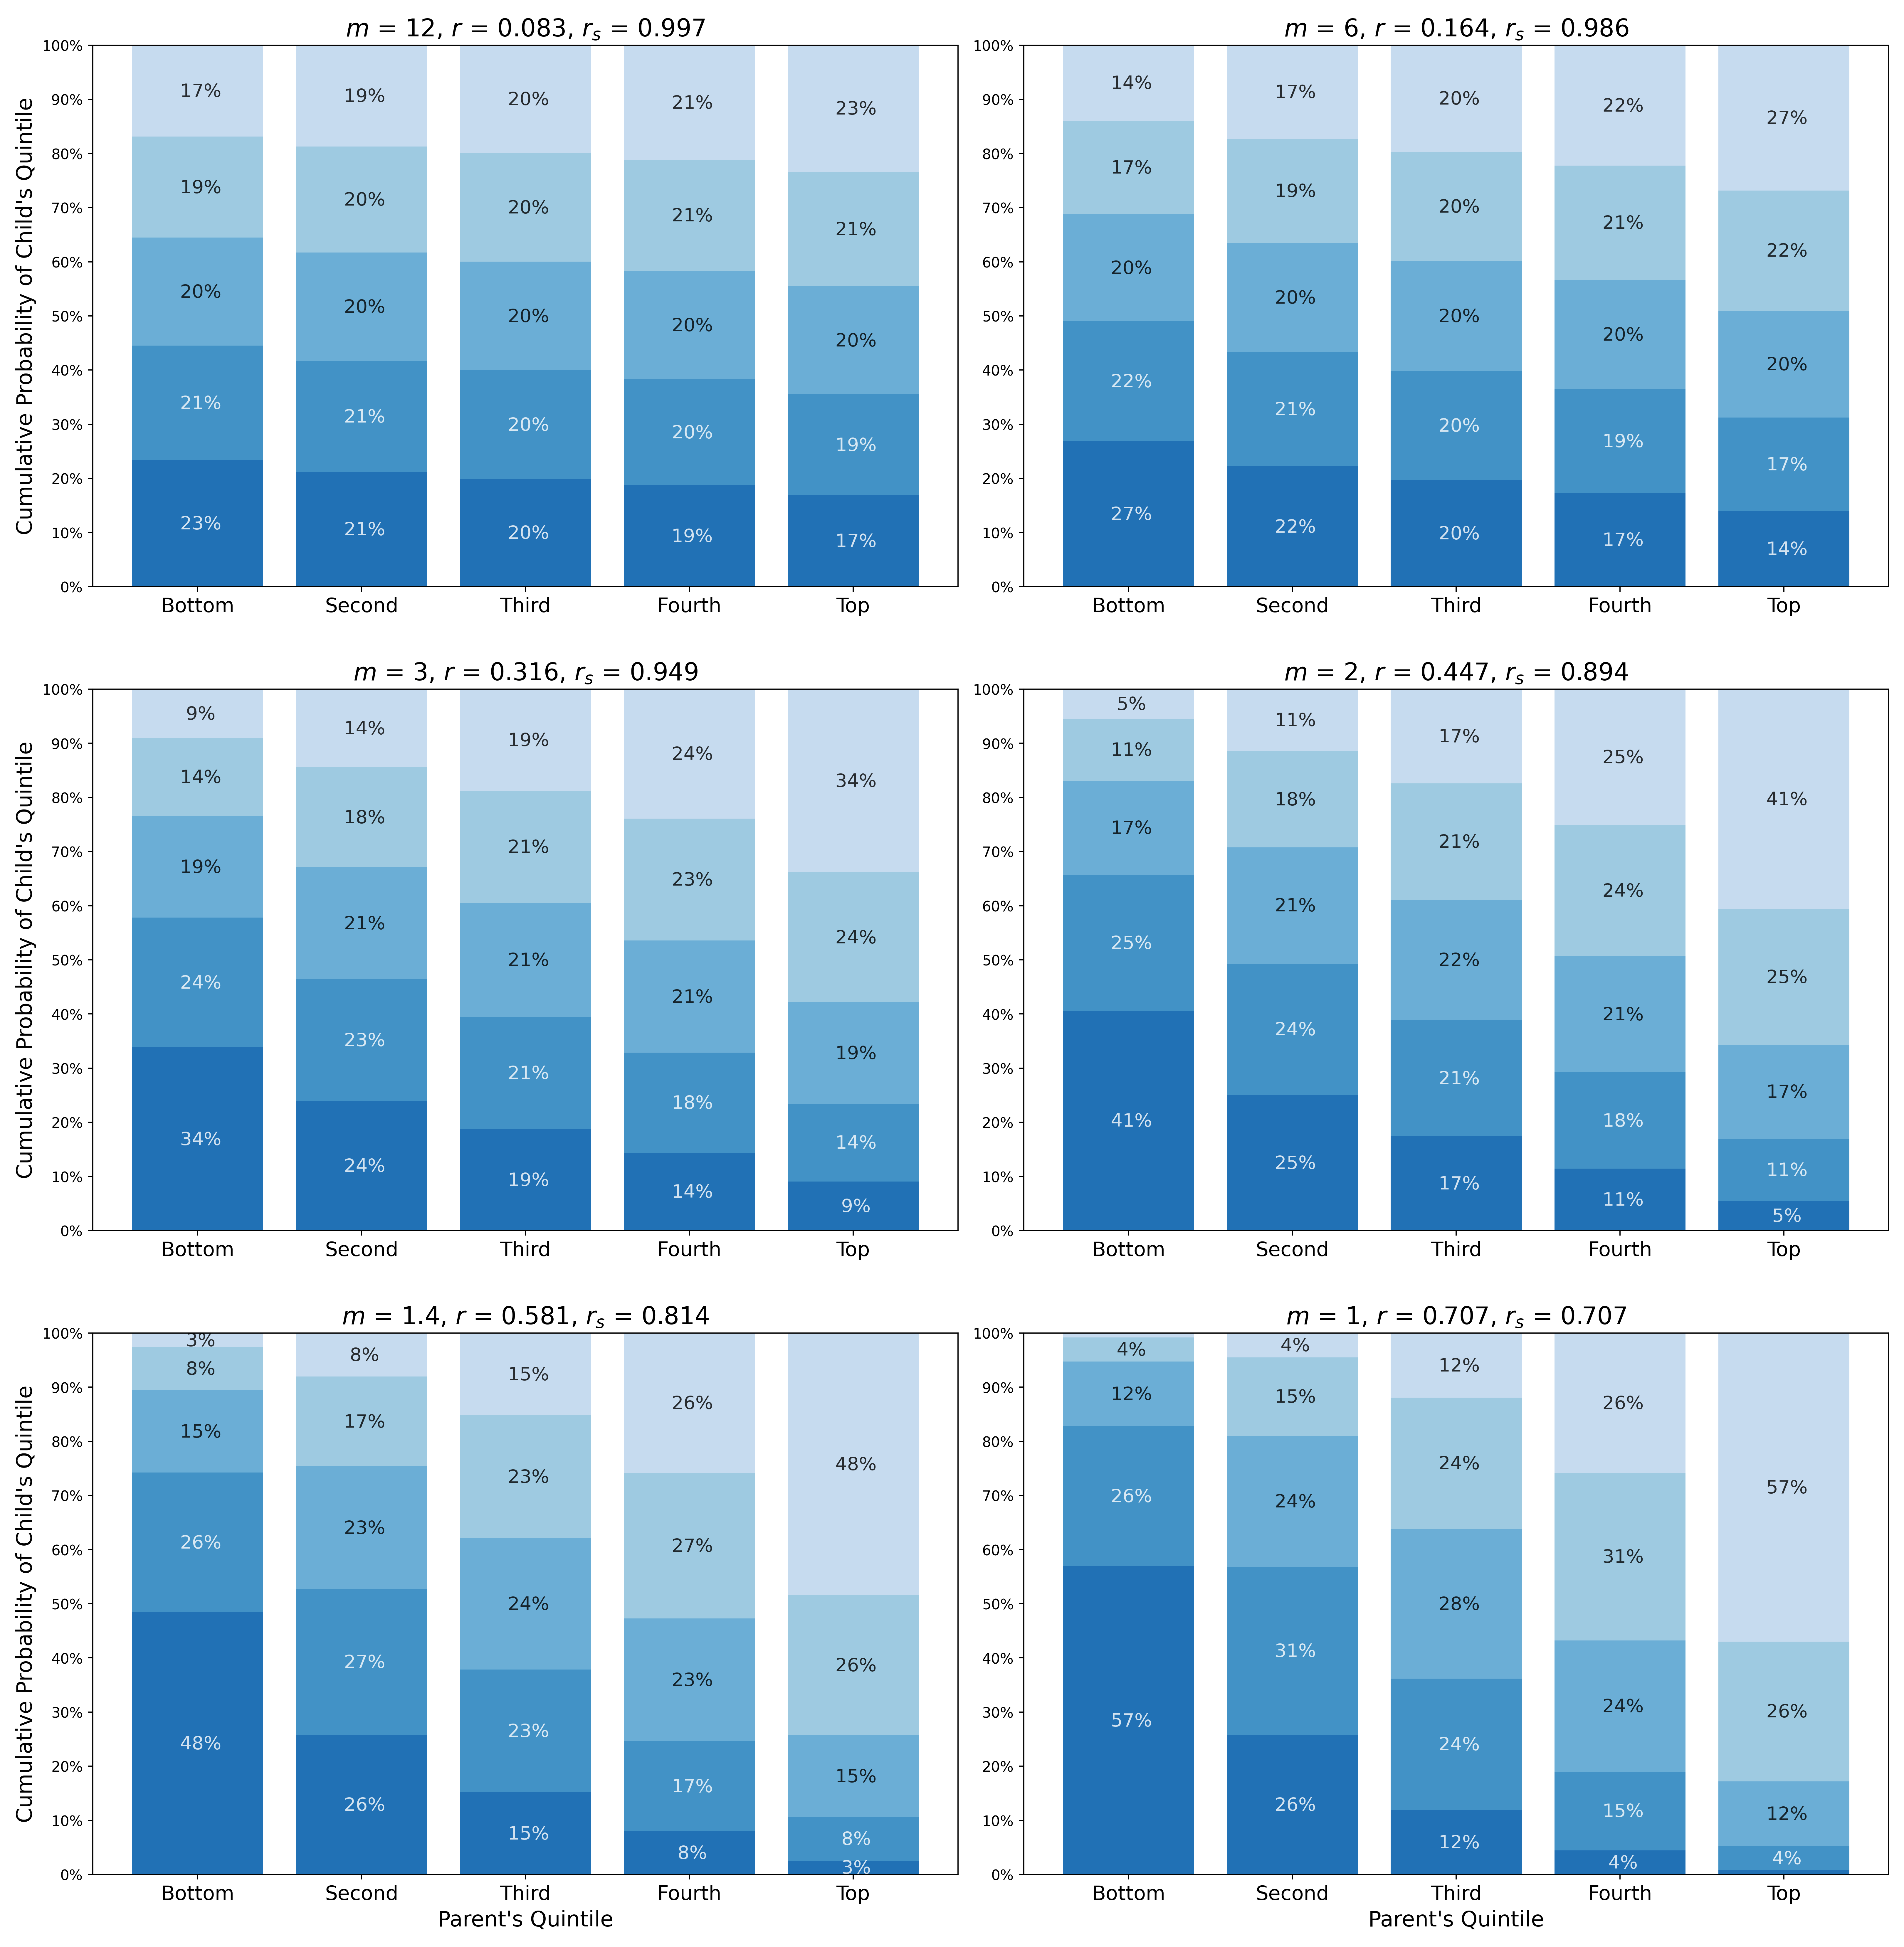
\includegraphics[width=5.2in]{figures/quintile-mobility.png}
\caption{Parent-to-child quintile transition matrices, over decreasing levels of mobility, with SPV.}
\label{fig:quintile_mobility}
\end{figure}



\begin{figure}[H]
\centering
%\advance\leftskip-0.4in
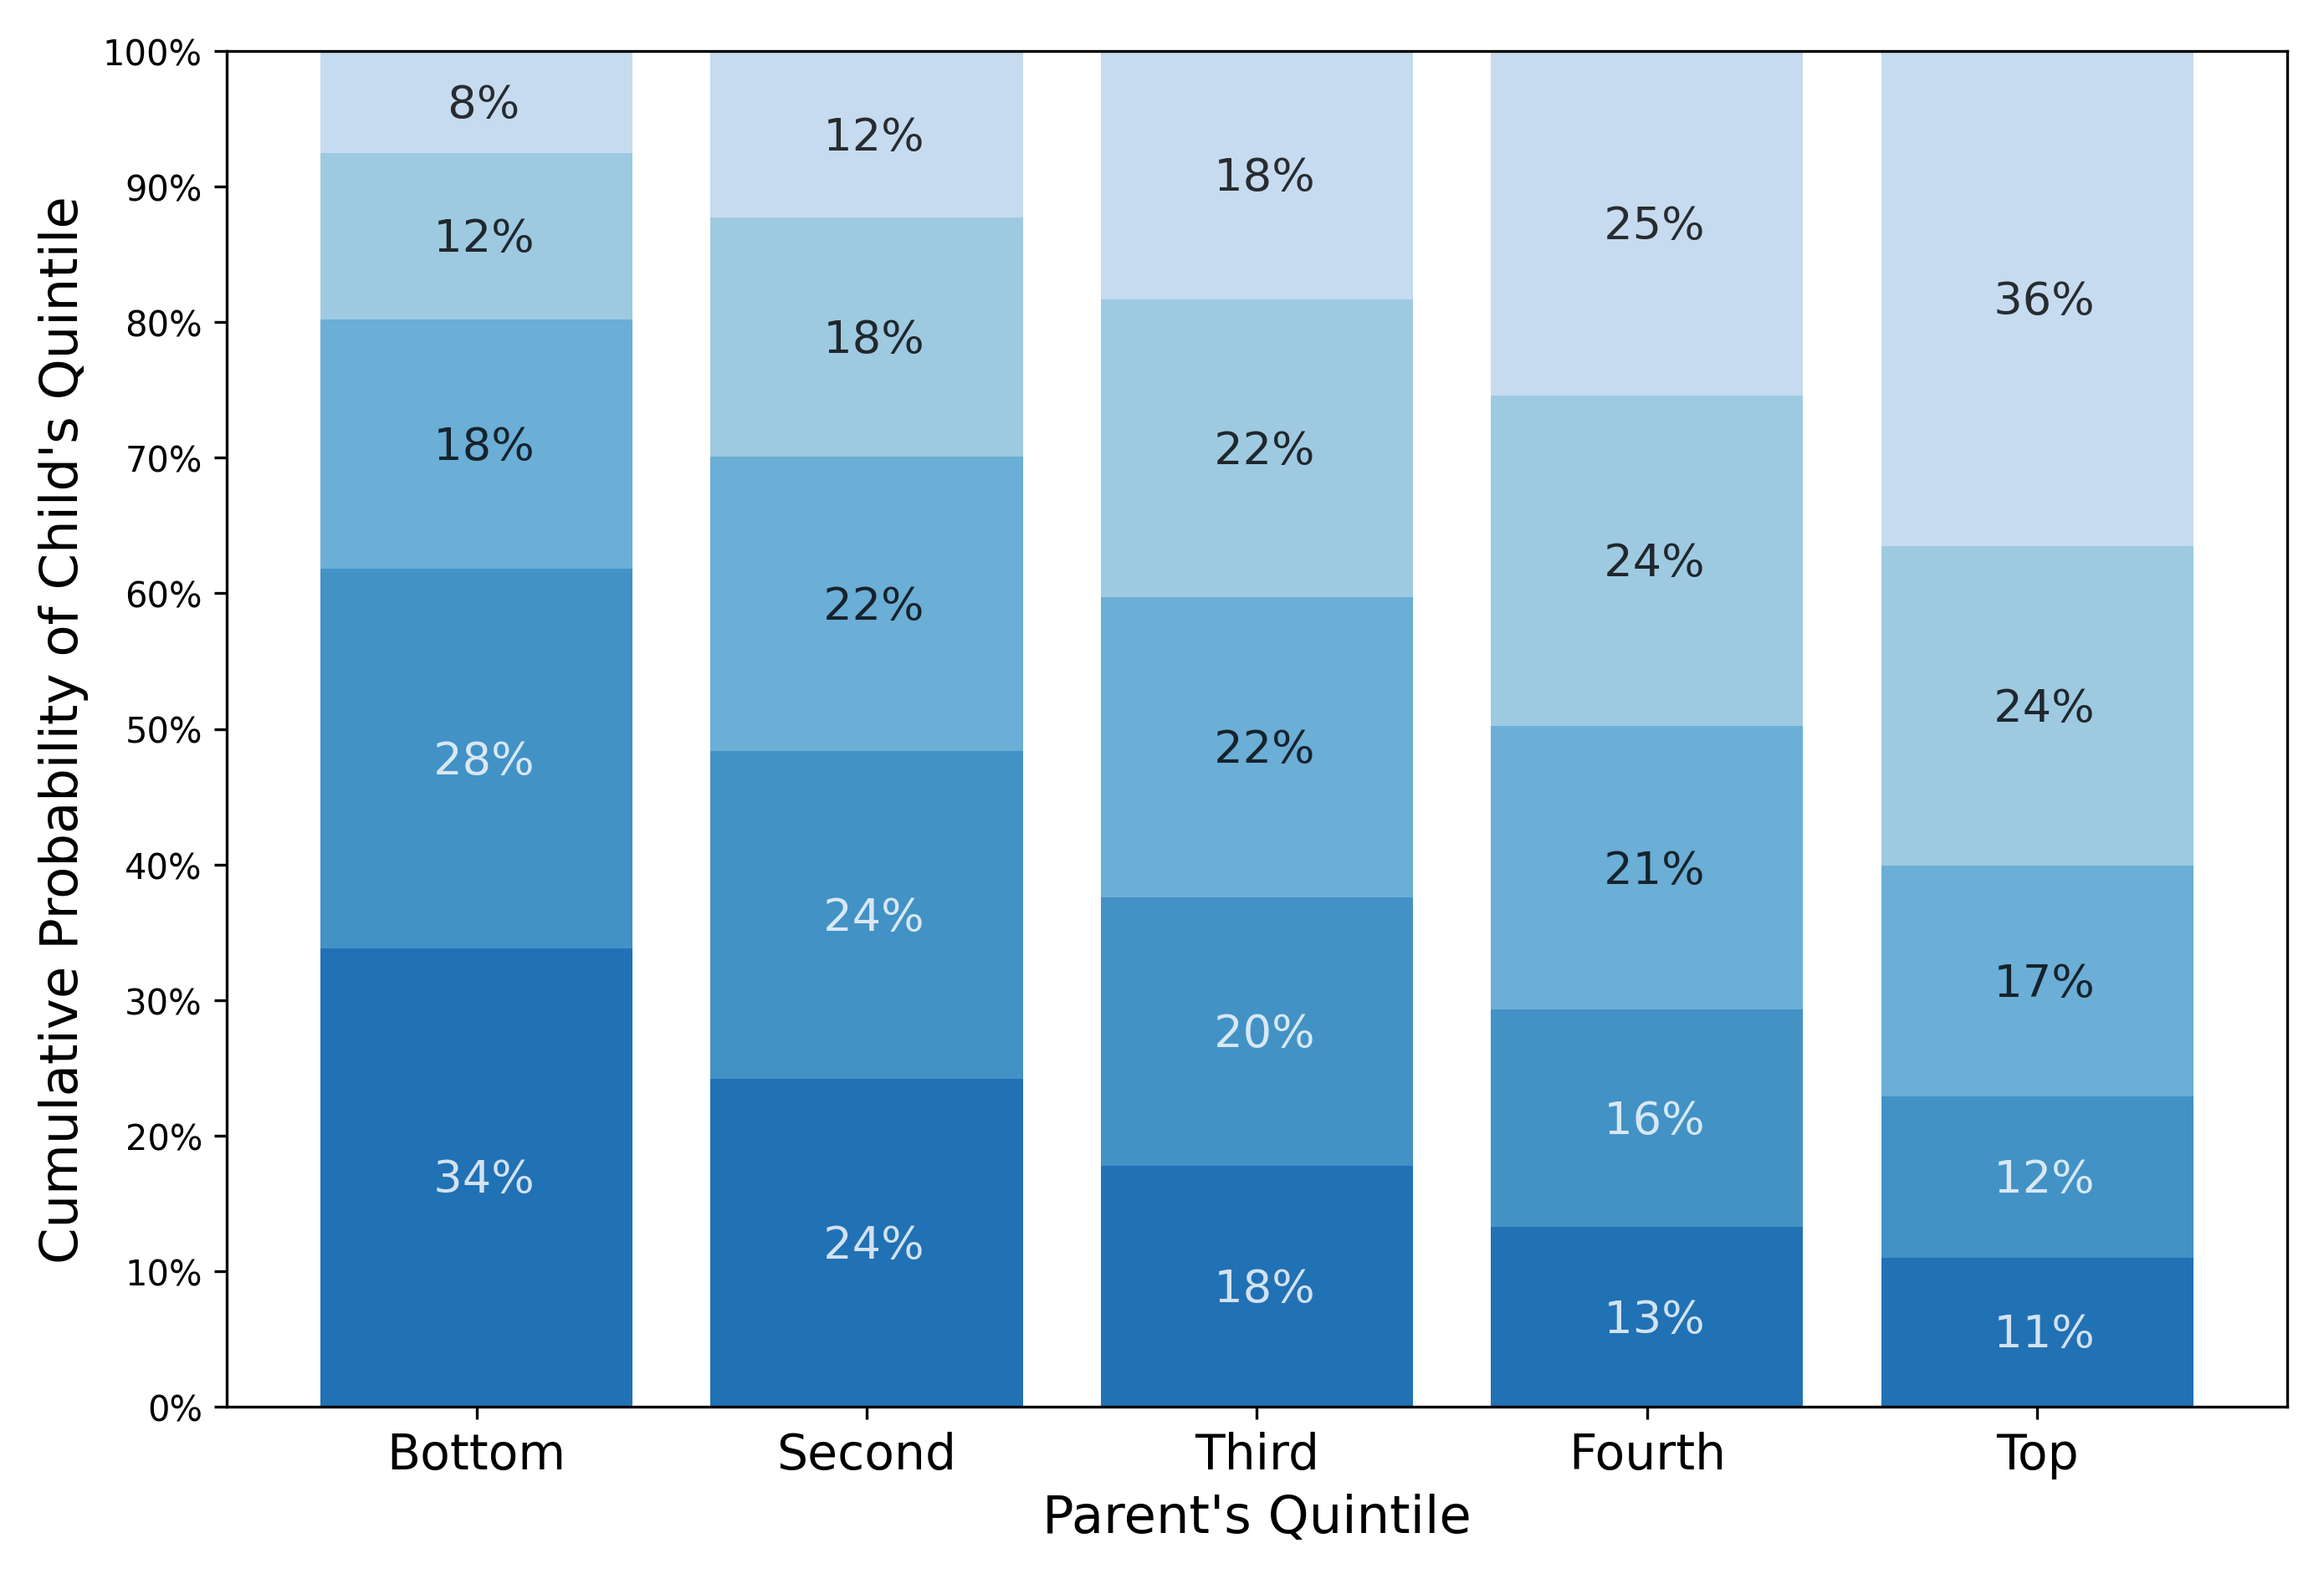
\includegraphics[width=2.8in]{figures/quintile-chetty.png}
\caption{Parent-to-child quintile transition matrix for US family income data for the 1980-82 birth cohort \cite{chetty}.}
\label{fig:quintile_chetty}
\end{figure}



% DISCUSSION
\section{Discussion}

The model proposed in this paper extends the normal linear model (linear regression with normally distributed residuals) into a Markov model. The initial state is a normal distribution, and all states after that are also normally distributed. It has immediate application to a polygenic trait such as height, which is normally distributed, and for which normal linear models have are an established method of predicting adult child height from parent height \cite{luo}.

\subsection{Model Properties}

Under a linear model, the conditional expectation for a child's score is the weighted average of the parent's score and the mean population score, where the weight of the parent's score is given by the regression coefficient $r$. Around this expectation, or prediction, there is random normal variation with an SD that is assumed in the model to be proportional to the marginal SD of the parent-generation population, where the degree of proportionality is given by the residual coefficient $s$.

This simple formulation relating parents and their children is re-applied through induction as generations reproduce in successive generations. The result is a Markov model in discrete time (generations) and continuous space (phenotypic score). From this model, conditional normal distributions are derived for the scores of descendants and ancestors of any generation-gap $n$ apart. Furthermore, the conditional distribution of an ancestor or descendant's score follows an exponential function of convergence to population distributions as $n$ increases, with rate constants determined by $r$ and $s$. That is, as the distance to a descendant or ancestor increases, predictive information is lost as an exponential function of the generation-gap.

The simple formulation is also consistent with the overall normal distribution of the polygenic trait in the population. Assuming the initial generation is normally distributed, all future and past generations are also normally distributed. To obtain the marginal distribution of the child's generation, the RV representing a parent---scaled by the regression coefficient, is combined additively with the standard normally distributed RV representing the variation about the prediction---scaled by the residual coefficient. The sum of independent normally distributed RVs is a normal RV with expectation equal to the sum of the expectations and variance equal to the sum of the variances. An immediate result is therefore that the population variance of the child-generation is proportional to that of the parent-generation by $r^2 + s^2$. This means that for there to be constant population variance between generations (SPV), $r^2 + s^2$ must equal one.

SPV results in the stationary distribution. That is, the conditional descendant and ancestor distributions are identical for the same generation-gap $n$. Equivalently, the system behaves the same with time going forwards or backward. When scores are indexed by percentile (relative to the population of their generation) the Markov chain is stationary and reversible in all cases (for both stable and unstable population variance). This is because indexing by percentile standardizes the differing population variances of the generations. Reversibility means that predicting a child's or grandchild's score has the same form as predicting a parent's or grandparent's score (the CDD and CAD are the same).

\subsection{Intergenerational Edge Persistence}

Consider those with scores on the edge of the population distribution, where the edge boundary is defined by some threshold. What proportion of these members (e.g. the tallest members of the population) are the children of parents also above the threshold (e.g. the tallest members of the last generation)? There are two counteracting effects: probability and number. Parents above the threshold have a higher probability of having children also above the threshold. However, there are many parents from the rest of the distribution whose children can end up above the threshold. The amount of edge persistence thus results from a competition of sorts between the greater probability for the tall parents and the greater number of shorter parents. Intuitively, when mobility ($m$) is greater, there is less edge persistence and vice versa. These questions can be answered for quintiles from the visualizations in section \ref{visuals}, and the software is available to examine other thresholds (see section \ref{links}).


\subsection{Potential to Model Genetic and Environmental Factors}

The observed approximation of the log-normal distribution to income (Figs. \ref{fig:quintile_mobility} and {\ref{fig:quintile_chetty}) suggests an application of the model to this domain. That is, a person's income could result from the multiplicative combination of many factors that correlate between parents and children. Then, a person's log-income would be normally distributed due to the central limit theorem, as with height, and his or her adult child's log-income could be predicted with a normal linear model.

The example of US family income introduced in the section on visualizations of percentile transition matrices suggests that a normal linear model may be useful to describe the relation between parents and their children for a trait with genetic or environmental determinants, or a combination thereof. This is especially reasonable to expect if the effects of the environment are also numerous and, on average, small, as are the effects of genes for a polygenic trait. Then, the trait should be normally distributed in the population and might fall under the paradigm of the linear model, in which conditional expectation for a child's score is a weighted average (by $r$) of the parent's score and the mean population score.

\subsection{Future Work}

In future work, the Markov model described in this paper could model traits that are approximately normally distributed and for which child scores can be predicted from parent scores with a normal linear model. These traits could have some arbitrary combination of genetic or environmental determinants, as long as they meet those basic two requirements. For these traits, this paper introduces a vocabulary of sorts: the regression coefficient $r$ and the residual coefficient $s$. Estimates of the mobility measure could enable a standard comparison between the mobility of these traits, such as between height and income as discussed here.


Additional future work could apply the multi-generational extension of the normal linear model shown in this paper to other generalized linear models. This extension was justified for describing a population that reproduces between generations, in which the forward one-step transition between generations is well-modeled by a normal linear relationship. However, other general linear models, such as the Poisson or the Gamma, might also be extended to a Markov model, with potential applications as well. Lastly, this paper described a univariate polygenic trait. It may be interesting to explore a multivariate normal linear Markov model, which could model a set of related polygenic traits with non-zero covariances.


%% PROBABILITY KERNELS %%
\section{Appendix 1. Probability Kernels}

Probability kernels consist of state-to-set and set-to-set kernels, which can be given conditionally as attributable and destined kernels that form the building blocks of percentile transition matrices.

\subsection{State and Set Kernels}

\begin{definition}
Let the probability kernel $P_n(D, x_i)$ be the $n$-step probability of reaching the set $D \subseteq \mathbb{R}$ in the descendant population from the state $x_i$ in the ancestor population, given by
\begin{equation}
P_n(D, x_i) = \int_{x_{i+n}\in D}^{} f_d(x_{i+n}|x_i)f_m(x_i) \, dx_{i+n}
\label{eq:state_set}
\end{equation}
where $f_d(x_{i+n}|x_i)$ is the conditional probability density function (pdf) of the CDD (Eq. \ref{eq:d_dist}) and $f_m(x_i)$ is the pdf of the marginal distribution (Eq. \ref{eq:pop_dist}).
\label{def:state_set}
\end{definition}

If $D$ is an uninterrupted set $(D_{min}, D_{max})$, Def. \ref{def:state_set} can be simplified to
\begin{equation}
P_n(D, x_i) = f_m(x_i)[\, \Phi(\frac{D_{max}- \tilde{\mu}_{i+n}}{\tilde{\sigma}_{i+n}}) - \Phi(\frac{D_{min}- \tilde{\mu}_{i+n}}{\tilde{\sigma}_{i+n}}) \, ]
\end{equation}
where $\Phi$ is the standard normal cumulative density function (cdf).


\begin{definition}
Let the probability kernel $P_n(D, A)$ be the $n$-step probability of reaching the set $D \subseteq \mathbb{R}$ in the descendant population from the set $A \subseteq \mathbb{R}$ in the ancestor population, given by
\begin{equation}
P_n(D, A) = \int_{x_i\in A}^{} P_n(D, x_i) \, dx_i \ .
\label{eq:set_set}
\end{equation}
\label{def:set_set}
\end{definition}


\subsection{Kernel Reversibility}

Under reversibility, we have
\begin{equation}
f_d(x_{i+n}|x_i)f_m(x_i) = f_d(x_i|x_{i+n})f_m(x_{i+n})
\end{equation}
$\forall i, n \in \mathbb{N}$, and $\forall x_{i}, x_{i+n} \in \mathbb{R}$, which means by Eqs. \ref{eq:state_set} and \ref{eq:set_set} we have
\begin{equation}
P_n(D, A) = P_n(A, D)
\label{eq:set_set_eq}
\end{equation}
$\forall A, D \subseteq \mathbb{R}$.

It should also be noted that when $A$ and $D$ are percentile sets (described in section \ref{formulation}), Eq. \ref{eq:set_set_eq} holds even under unstable population variance because the values are normalized to the differing variances of the two generations. This results in the persymmetry property of percentile transition matrices.


% ATTRIBUTABLE
\subsection{Attributable and Destined Kernels}

\begin{definition}
Let $P_{\alpha , n}(A | D)$ be the conditional probability that a state $X_{i+n} \in D \subseteq \mathbb{R}$ is descendant from (attributable to) a state $X_i \in A \subseteq \mathbb{R}$, given by
\begin{equation}
P_{\alpha , n}(A | D) = \frac{P_n(D, A)}{P_n(D)} \ ,
\label{eq:attributable}
\end{equation}
where $P_n(D)$ is the marginal probability of $X_{i+n} \in D$ (see Eq. \ref{eq:pop_dist}).
\label{def:destined}
\end{definition}

% DESTINED

\begin{definition}
Let $P_{\delta , n}(D | A)$  be the conditional probability that a state $X_i \in A \subseteq \mathbb{R}$ is ascendant from a state $X_{i+n} \in D \subseteq \mathbb{R}$ (i.e. $X_{i+n}$ is destined for $D$), given by
\begin{equation}
P_{\delta , n}(D | A) = \frac{P_n(D, A)}{P_i(A)} \ ,
\label{eq:destined}
\end{equation}
where $P_i(A)$ is the marginal probability of $X_i \in A$ (see Eq. \ref{eq:pop_dist}).
\label{def:attributable}
\end{definition}


\section{Appendix 2. Software and Statistical Tests} \label{links}
The software for calculating and estimating the probability transition matrices (section \ref{visuals}) and the full analysis of the English data (section \ref{pearson}) are both available with extensive documentation at \href{https://github.com/jessebmurray/polygenic}{https://github.com/jessebmurray/polygenic}. The results from these sections can be fully reproduced using this repository.


% BIBLIOGRAPHY
\begin{thebibliography}{6}

\bibitem {battistin}
Battistin, E., Blundell, R., and Lewbel, A. (2007).
\newblock Why is consumption more log normal than income? Gibrat's law revisited.
\newblock {\em Battistin, E. and Blundell, R. and Lewbel, A. (2009). Journal of Political Economy}, 117(6), 1140-1154. \url{doi:10.1086/648995}

\bibitem{bogin}
Bogin, B. and Rios, L. (2003).
\newblock Rapid morphological change in living humans: implications for modern
  human origins.
\newblock {\em Comparative Biochemistry and Physiology Part A: Molecular and
  Integrative Physiology}, 136(1):71---84.

\bibitem {chetty}
Chetty, R., Hendren, N., Kline, P., and Saez, E. (2014).
\newblock {Where is the land of Opportunity? The Geography of Intergenerational
  Mobility in the United States}.
\newblock {\em The Quarterly Journal of Economics}, 129(4):1553--1623.

\bibitem {karlberg}
Karlberg, J. and Albertsson-Wikland, K. (1995).
\newblock Growth in full- term small-for-gestational-age infants: From birth to
  final height.
\newblock {\em Pediatric Research}, 38:733--739.

\bibitem {krapohl}
Krapohl, E. and Plomin, R. (2016).
\newblock Genetic link between family socioeconomic status and children's educational achievement estimated from genome-wide snps.
\newblock {\em Molecular Psychiatry}, 21(3):437--443.

\bibitem {lange_article}
Lange, K. (1997a).
\newblock An approximate model of polygenic inheritance.
\newblock {\em Genetics}, 147(3):1423--1430.

\bibitem {lange_book}
Lange, K. (1997b).
\newblock {\em The Polygenic Model. In: Mathematical and Statistical Methods
  for Genetic Analysis. Statistics for Biology and Health}.
\newblock Springer, New York, NY.

\bibitem {luo}
Luo, Z.~C., Albertsson-Wikland, K., and Karlberg, J. (1998).
\newblock Target height as predicted by parental heights in a population-based
  study.
\newblock {\em Pediatric Research}, 44(4):563--571.

\bibitem {neal}
Neal, D. and Rosen, S. (1998).
\newblock Theories of the distribution of labor earnings.
\newblock Working Paper 6378, National Bureau of Economic Research.

\bibitem {pearson}
Pearson, K. and Lee, A. (1903).
\newblock On the laws of inheritance in man: I. inheritance of physical
  characters.
\newblock {\em Biometrika}, 2(4):357--462.

\bibitem {perkins}
Perkins, J.~M., Subramanian, S.~V., Davey~Smith, G., and Özaltin, E. (2016).
\newblock Adult height, nutrition, and population health.
\newblock {\em Nutrition reviews}, 74(3):149--165.

\bibitem {preece}
Preece, M.~A. (1996).
\newblock The genetic contribution to height.
\newblock {\em Hormone Research in Pediatrics}, 45(Suppl. 2):56--58.

\bibitem {rieger}
Rieger, R., Michaelis, A., and Green, M. (1968).
\newblock {\em A Glossary of Genetics and Cytogenetics}.
\newblock Springer, New York, NY.

\bibitem {trzaskowski}
Trzaskowski, M., Harlaar, N., Arden, R., Krapohl, E., Rimfeld, K., McMillan,
  A., Dale, P.~S., and Plomin, R. (2014).
\newblock Genetic influence on family socioeconomic status and children's
  intelligence.
\newblock {\em Intelligence}, 42(100):83---88.

\bibitem {wood}
Wood, A.~R. and Esko, T., e.~a. (2014).
\newblock Defining the role of common variation in the genomic and biological
  architecture of adult human height.
\newblock {\em Nature Genetics}, 46(11):1173--1186.

\bibitem {yengoetal} Yengo, L.,  Sidorenko, Julia, Kemper, Kathryn E,  Zheng, Zhili,  Wood, Andrew R,   Weedon, Michael N,  Frayling, Timothy M.,  Hirschhorn, Joel,  Yang, Jian,  Visscher, Peter M., the GIANT Consortium (2018). 
    \newblock Meta-analysis of genome-wide association studies for height and body mass index in ~700000 individuals of European ancestry.
    \newblock {\em  Human Molecular Genetics,} 27(20):3641--3649. \url{https://doi.org/10.1093/hmg/ddy271}

\end{thebibliography}

\end{document}
